\documentclass[10pt, english]{report}

\usepackage{hyperref}

\usepackage{float}

\usepackage{subcaption}
\usepackage[export]{adjustbox}
\usepackage{wrapfig}
%encoding
%--------------------------------------
\usepackage[utf8]{inputenc}
\usepackage[T1]{fontenc}
%--------------------------------------

%French-specific commands
%--------------------------------------
\usepackage{babel}
\usepackage[autolanguage]{numprint}
%--------------------------------------

%Hyphenation rules
%--------------------------------------
\usepackage{hyphenat}
\hyphenation{mathéma-tiques récu-pérer}
%--------------------------------------

%Maths box
%--------------------------------------
\usepackage{amsmath}
\usepackage[most]{tcolorbox}

\tcbset{colback=yellow!10!white, colframe=red!50!black, 
	highlight math style= {enhanced, %<-- needed for the ’remember’ options
		colframe=red,colback=red!10!white,boxsep=0pt}
}
%--------------------------------------

%code blocs
%--------------------------------------

\usepackage{listings}
\usepackage{xcolor}

\usepackage{multirow}
\usepackage{makecell}
\usepackage{booktabs}
\usepackage{hhline}
\usepackage{arydshln}
\usepackage{tablefootnote}
\usepackage[numbers]{natbib}

\setlength\heavyrulewidth{0.25ex}

\def\BibTeX{{\rm B\kern-.05em{\sc i\kern-.025em b}\kern-.08em
    T\kern-.1667em\lower.7ex\hbox{E}\kern-.125emX}}
    

\definecolor{codegreen}{rgb}{0,0.6,0}
\definecolor{codegray}{rgb}{0.5,0.5,0.5}
\definecolor{codepurple}{rgb}{0.58,0,0.82}
\definecolor{backcolour}{rgb}{0.95,0.95,0.92}

\lstdefinestyle{mystyle}{
	backgroundcolor=\color{backcolour},   
	commentstyle=\color{codegreen},
	keywordstyle=\color{magenta},
	numberstyle=\tiny\color{codegray},
	stringstyle=\color{codepurple},
	basicstyle=\ttfamily\footnotesize,
	breakatwhitespace=false,         
	breaklines=true,                 
	captionpos=b,                    
	keepspaces=true,                 
	numbers=left,                    
	numbersep=5pt,                  
	showspaces=false,                
	showstringspaces=false,
	showtabs=false,                  
	tabsize=2
}

\lstset{style=mystyle}
%--------------------------------------

\usepackage[margin=2cm]{geometry}
\usepackage{graphicx}

\title{
	
\includegraphics[scale=1]{img/logo.png}\\[4cm]
	\huge\textbf{Natural Language Processing for Fact-Checking and Claim Assessment}\\[3cm]
}
\author{
	Othman EL HOUFI\\
	Dimitris KOTZINOS \\[0.5cm]
	\textbf{MSc Research in Data Science \& Machine Learning} \\[2cm]
}

\date{\today}

\begin{document}
	
	%%%%%TITLE%%%%%
	\begin{titlepage}
		\maketitle
	\end{titlepage}

\chapter*{Abstract}
As false information and fake news are propagating throughout the internet and social networks, the need of fact-checking operations becomes necessary in order to maintain a truthful digital environment where general information can be reliably exploited whether in politics, finance or other domains. The need of this online claim assessment comes from the fact that fake news and false information can have a big negative impact on politics, economy (2016 USA Elections) and public health (COVID-19).\\ 
A number of solutions have been proposed to deal with this problem and limit the spread of false information, both manual and automatic. Of course the manual approaches done on websites such as \textit{PolitiFact.com}, \textit{FactCheck.org} and \textit{Snopes.com} don't construct a viable solution for the long term as the speed and scale of information propagation increase exponentially rendering this manual fact-checking operation where human fact-checkers can't scale up at the same rate limited and incapable of solving the problem.\\
Here, we present our contribution in this regard: an automated solution for fact-checking using FEVER dataset as a source of truth and a state of the art language models used today for NLP tasks (BERT, RoBERTa, XLNet...) in order to classify a given claim as \textit{Supports}, \textit{Refutes} or \textit{Not enough information (NEI)}. We successfully prove that fine-tuning a LM with the correct settings can achieve an accuracy of 62\% and F1-score of 61\% which is better than the majority of fact-checking methods that exists today.\\[1cm]

\textbf{Keywords:} Natural Language Processing, Language Model, Wikipedia, Fine-tuning, Zero-shot Learning, Text processing, Natural Language Inferencing, Fact-Checking, Fake-news.

%%%%%TABLE OF CONTENT%%%%%
\tableofcontents

\chapter{Introduction}
\section{Project Context}

From a social and psychological perspective, humans have been proven irrational and vulnerable when differentiating between truth and false news (typical accuracy ranges between 55\% and 58\%) \cite{zhou2019fake}, thus fake news obtain public trust relatively easier than truthful news because individuals tend to trust fake news after constant exposure (\textit{Validity effect}), or if it confirms their pre-existing beliefs (\textit{Confirmation bias}), or simply due to the obligation of participating socially and proving a social identity (\textit{Peer pressure}). The social sciences are still trying to comprehend the biological motivations that makes fake news more appealing to humans.\\

On the other hand, the growth of social media platforms resulted in a huge acceleration of news spreading whether true or false. As of Aug. 2017, 67\% \cite{zhou2019fake} of Americans get their news from social media. These platforms even give the user the right to share, forward, vote and participate to online discussions. All of this made the problem of fake news spreading more and more dangerous, our economies for example, are not robust to the spread of falsity, false rumors have affected stock prices and the motivations for large-scale investments, as we witnessed after a false tweet claimed that Barack Obama was injured in an explosion which caused \$130 billion drop in stock value \cite{vosoughi2018spread}. Another recent example is related to public health where rumors about COVID-19 vaccines and drug companies influenced people in their decision on getting vaccinated.\\

That being said, is there a way to monitor the spread of fake news through social media? Or more specifically, how can we differentiate between fake news and truthful news, and at what level of confidence can we do that?\\

From a computer engineering perspective, various approaches were examined:

\begin{itemize}
\item \textbf{Knowledge-based Fake News Detection \cite{chernyavskiy2021whatthewikifact}:} a method aims to assess news authenticity by comparing the knowledge extracted from to-be verified news content with known facts, also called fact-checking.
\item \textbf{Style-based Fake News Detection \cite{przybyla2020capturing}:} focuses on the style of writing, i.e. the form of text rather than its meaning.
\item \textbf{Propagation-based Fake News Detection \cite{shu2020hierarchical}:} a principled way to characterize and understand hierarchical propagation network features. We perform a statistical comparative analysis over these features, including micro-level and macro-level, of fake news and true news.
\item \textbf{Credibility-based Fake News Detection \cite{sitaula2020credibility}:} the information about authors of news articles can indicate news credibility and help detect fake news.
\end{itemize}

In this paper we will focus on a modern approach that utilizes Language Models (LMs) for fact-checking. The goal is not to implement an algorithm that scans social networks for real time fake news detection, but rather we will design a model that can assess with a degree of confidence the truthfulness or falseness of a claim given by a user as an input by exploiting LMs that were already trained on Wikipedia, and fine-tune each LM for a downstream task in order to solve this classification problem.

\section{Use case scenario}
Suppose that while browsing the internet or talking to people you come across a claim that says \textit{"The former U.S president John F. Kennedy died in September 22, 1963"}, as it is a general truth and not a relative truth it should be easier to verify the validity of this claim as well as find evidence that proves it.\\
Using our algorithm, you can simply write the claim you like to verify with no regards to a specific linguistic rule as an input, the model will assess if the claim is True, False, or Not Enough Information as well as giving a percentage of confidence and evidence of the results that were processed straight from Wikipedia's database.\\
Coming back to our example, the model should return that \textit{"John F. Kennedy died in November 22, 1963"} so the input claim is false.\\

During this project we created an algorithm that can only classify claims, and in a future work the algorithm will be able to provide detailed explanations and evidences of the classified claim.

\section{Tools used}

\chapter{Potential Datasets}
The rise of fake news in the internet created the need of setting-up databases that contains as much claims as possible checked and approved manually by journalists and fact-checkers worldwide in order to be used as a dataset for experiments in automatic fact-checking models or just simply to be a reference to other journalists and the general public.

\section{FEVER dataset \cite{thorne2018fever}}
\label{sec:fever}
FEVER (Fact Extraction and VERification) consists of 185,445 claims generated by altering sentences extracted from Wikipedia and subsequently verified without knowledge of the sentence they were derived from. The claims are classified as Supported, Refuted or NotEnoughInfo. For the first two classes, the annotators also recorded the sentence(s) forming the necessary evidence for their judgment\cite{thorne2018fever}.

\begin{figure}[H]
	\centering
	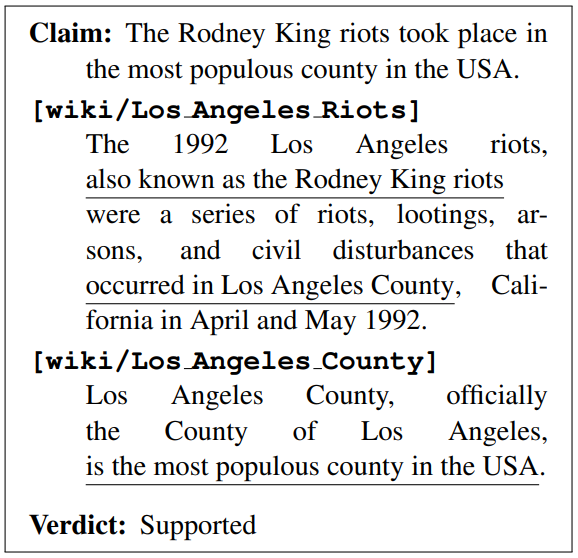
\includegraphics[scale=0.4]{img/fever_example.png}
	\caption{Manually verified claim requiring evidence from multiple Wikipedia pages.}
\end{figure}

\section{CREDBANK dataset \cite{mitra2015credbank}}
The \textit{CREDBANK} corpus was collected between mid October 2014 and end of February 2015. It is a collection of streaming tweets tracked over this period, topics in this tweet stream, topics classified as events or non events, events annotated with credibility ratings.the \textit{CREDBANK} Dataset comprises more than 60M tweets grouped into 1,049 real-world events, each annotated by 30 human annotators. The label labeling of each tweet is a vector with 30 dimensions containing variable scores at five levels of veracity.

\section{LIAR dataset \cite{wang2017liar}}
\textit{LIAR} is a publicly available dataset for fake news detection. A decade-long of 12.8K manually labeled short statements were collected in various contexts from \textit{PolitiFact}, which provides detailed analysis report and links to source documents for each case. This dataset can be used for fact-checking research as well. Each statement is labeled on six levels: true, predominantly true, half-true, almost true, false, pants-fire.



\section{FAKENEWSNET dataset \cite{shu2018fakenewsnet}}
\textit{FakeNewsNet} is a multi-dimensional fake news data repository, which contains two comprehensive datasets that includes news content, social context, and dynamic information.

\begin{figure}[H]
	\centering
	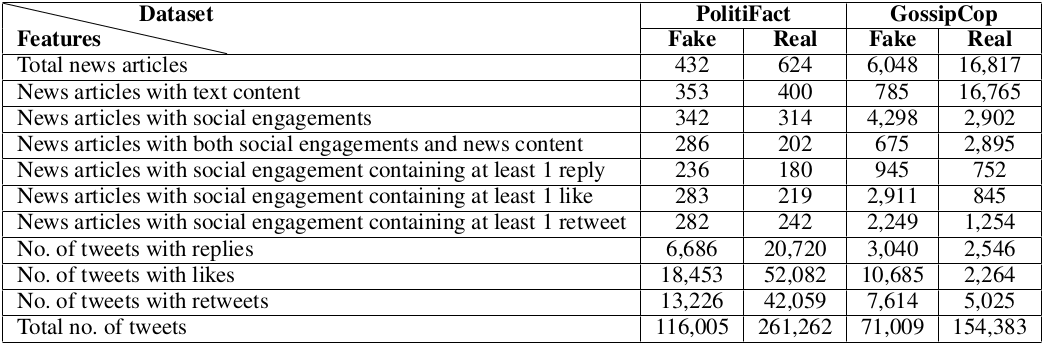
\includegraphics[scale=0.43]{img/fake_news_net_stats.png}
	\caption{Statistics of the FakeNewsNet repository \cite{shu2018fakenewsnet}}
\end{figure}

\begin{itemize}
\item \textbf{News content:} reliable news content retrieved from fact-checking websites and true news such as \textit{PolitiFact} and \textit{GossipCop}.
\item \textbf{Social context:} the user engagements related to the fake and real news pieces from fact-checking websites are collected using search application programming interfaces (API) provided by social media platforms such as the Twitter's Advanced Search API.
\item \textbf{Spatiotemporal information:} includes spatial and temporal information. For spatial information, we obtain the locations explicitly provided in user profiles. The temporal information indicates that we record the timestamps of user engagements, which can be used to study how fake news pieces propagate on social media, and how the topics of fake news are changing over time.
\end{itemize}

The multi-demnsionality of this dataset can be regarded as its strong value against previous datasets:

\begin{figure}[H]
	\centering
	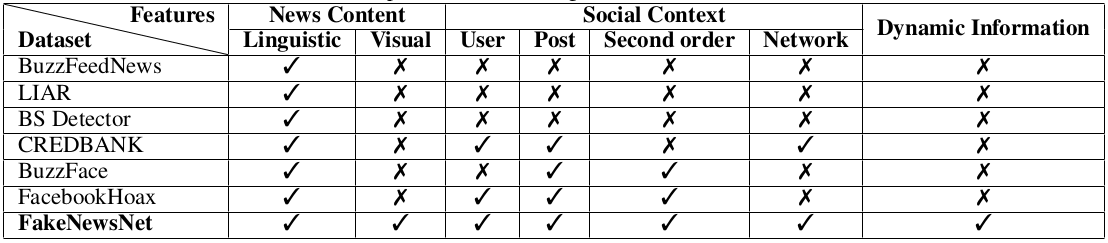
\includegraphics[scale=0.43]{img/fake_news_net_comparison.png}
	\caption{Comparison with existing fake news detection datasets \cite{shu2018fakenewsnet}}
\end{figure}

\newpage
\section{Other datasets and comparison \cite{de2021identifying}}
Of course other datasets exist with different structures and various sources. For each dataset we can conceptualize a new way of modeling classifiers, we can also use multiple datasets in one model.\\
 
\begin{figure}[H]
	\centering
	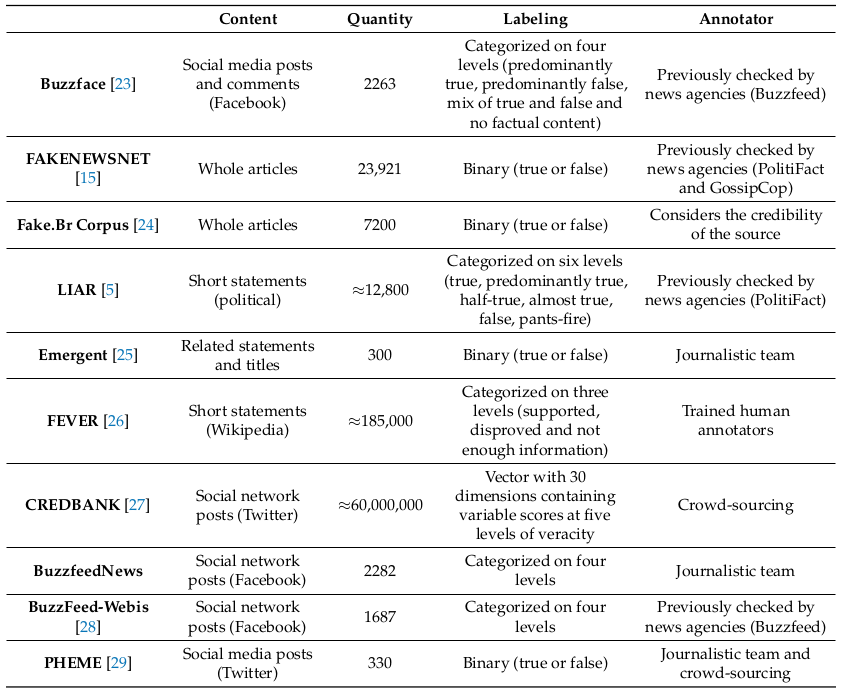
\includegraphics[scale=0.53]{img/datasets_comparison.png}
	\caption{Overview of fake news datasets available \cite{de2021identifying}}
\end{figure}


\chapter{Related work and solutions}
\section{Language model based fake news detection \cite{lee2020language} \cite{petroni2019language}}
A paper entitled \textit{"Language Models as Fact Checkers?"} published by a team from \textit{FacebookAI} and \textit{Hong Kong University of Science and Technology}, provides an example of a fact-checking model using zero-shot LM that outperforms a random baseline LM using the FEVER dataset\cite{thorne2018fever}.\\

The goal of fact-checking as mentioned previously, and relatively to this paper, is to validate the truthfulness of a given claim. Each claim is assigned to one of these labels: \textit{Supports}, \textit{Refutes} or \textit{Not enough information (NEI)} to verify.\\

This paper describes the difference between Traditional Pipeline fact-checking models and their zero-shot fact-checking LM:

\begin{itemize}
\item \textbf{Traditional pipeline:} this type of models access knowledge within an external knowledge base like Wikipedia in order to validate a claim. It involves information retrieval modules such as document retrieval and sentence retrieval.
\item \textbf{Zero-shot LM pipeline:} it replaces both the external knowledge base and the information retrieval modules with a pre-trained language model. In this case they used BERT as a pre-trained LM.
\end{itemize}

\begin{figure}[H]
	\centering
	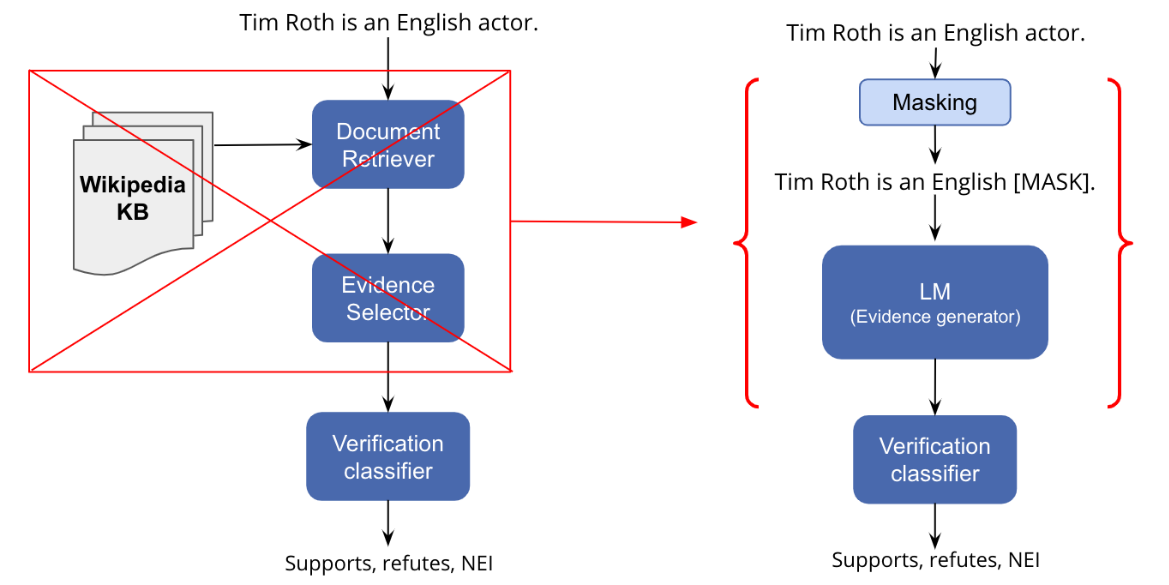
\includegraphics[scale=0.35]{img/tradition_and_zero_shot_lm.png}
	\caption{Traditional fact-checking pipeline (left) vs. zero-shot LM-based pipeline (right) \cite{lee2020language}}
\end{figure}

To implement this end-to-end fact-checking model, they started by using an \textbf{Automatic Masking} in order to mask the last named entity in the claim. This last named entity is identified using an off-the-shelf Named-Entity-Recognition (NER) model from spaCy. This ensures that the masked token makes use of the \textit{knowledge} encoded in a LM, otherwise a problem like stop-words masking can occur.\\
Next, they used \textbf{Verification by Entailment} in order to avoid naive matching predicted an gold tokens. This method leverages a textual entailment model from Al-lenNLP to validate the LM predictions.\\

\begin{figure}[H]
	\centering
	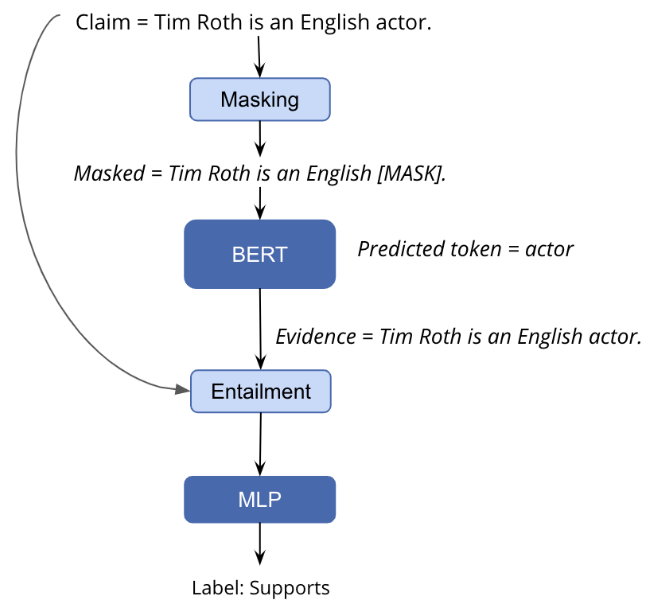
\includegraphics[scale=0.4]{img/LM_detailed_pipline.png}
	\caption{Detailed illustration of our pipeline \cite{lee2020language}}
\end{figure}

\begin{enumerate}
\item Masked the last named entity found by the NER model.
\item Get the top-1 predicted token from the LM, and fill in the [MASK] accordingly to create the "evidence" sentence.
\item Using the claim and generated "evidence" sentence, obtain entailment "features" using outputs from the last layer of the pre-trained entailment model (before the softmax).
\item Input the entailment features into a multi-layer perceptron (MLP) for final fact-verification prediction.
\end{enumerate}

\begin{figure}[H]
	\centering
	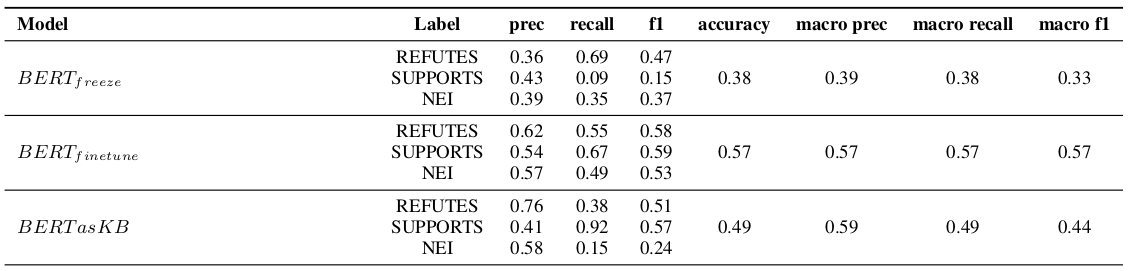
\includegraphics[scale=0.4]{img/bert_lm_evaluation.png}
	\caption{Performance comparison between BERT-as-encoder models ($BERT_{freeze}$ , $BERT_{finetune}$ ) and BERT-as-LM model ($BERTasKB$). \cite{lee2020language}}
\end{figure}

As for evaluation, they used precision, recall, F1 and accuracy metrics in order to compare the zero-shot LM with other baseline models. They observe that the proposed approach ($BERTasKB$) outperforms $BERT_{freeze}$ on all metrics suggesting that querying language models in QA style is a better approach for extracting their encoded knowledge. Similarly, $BERTasKB$ model achieves an accuracy score of 49\% which is comparable to Fever-baseline at 48.8\%, except without the need for explicit document retrieval and evidence selection.


\section{Styled based fake news detection \cite{przybyla2020capturing}}
A study done by \textit{Piotr Przybyła} named \textit{Capturing the Style of Fake News} in 2020 from Institute of Computer Science, Polish Academy of Sciences, in order to detect fake news or in other words assess the credibility of an article by looking at the style of writing rather than the meaning of the words and sentences.\\
The purpose of this study was to prove that general-purpose text classifiers, despite their good performance when evaluating simplistically, they overfit to sources of documents in training data. In contrast to this method, a truly style-based prediction that uses an analysis of the stylometric model shows that it focuses on sensational and affective vocabulary, known to be typical for fake news.\\

Fake news sources usually attempt to attract attention for short-time financial or political goal \cite{allcott2017social} rather than to build a long-term relationship with the reader, in this perspective, the language used by these sources tend to be informal, sensational and affective \cite{bakir2017fake}. This can be used to build a classifier for indicating low credibility.\\

First of all they started by gathering a corpus of 103,219 documents from 223 online sources labeled by media experts like \textit{PolitiFact} and \textit{Pew Research Center}. Then they designed two models: a neural network and a model based on features used in stylometric analysis. This has a purpose to demonstrate that the stylometric features based model captures the affective language elements.\\

\begin{figure}[H]
	\centering
	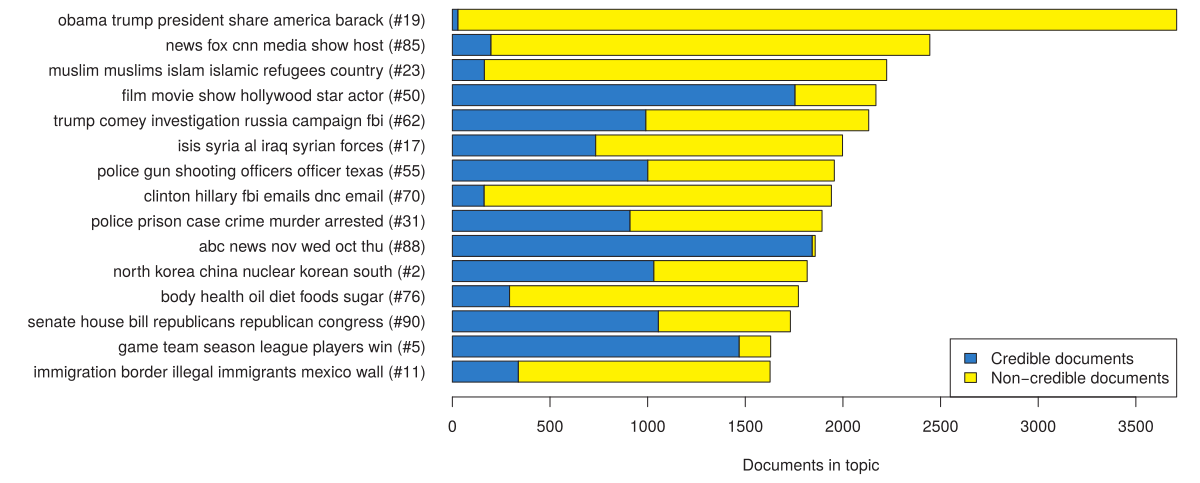
\includegraphics[scale=0.4]{img/documents_in_topic.png}
	\caption{The largest 15 LDA (Latent Dirichlet Allocation) topics in the corpus, each shown with the six most significant keywords, an identifier and bars illustrating number of credible and non-credible documents associated with it \cite{przybyla2020capturing}}
\end{figure}

\textbf{Stylometric classifier:} the architecture of this classifier is generally based on a collection of stylystic features followed by a linear modeling. The features are: 
	\begin{itemize}
	\item number of sentences, average sentence length (in words) and average word length (in characters),
	\item number of words matching different letter case schemes (all lower case, all upper case, just first letter upper case, other), represented as counts normalized by the document length,
	\item frequencies of POS uni-grams, bi-grams and trigrams, represented as counts normalized by the document length (if present in at least 5 documents),
	\item frequencies of words belonging to the 182 word categories in the expanded GI dictionary, represented as counts normalized by the document length.
	\end{itemize}

\textbf{Neural network classifier:} the applied solution was BiLSTMAvg a neural network with architecture based on elements used in natural language processing, i.e. word embeddings \cite{mikolov2013efficient} and bidirectional LSTM (Hochreiter and Schmidhuber 1997). The following layers are included:
	\begin{itemize}
	\item An embedding layer, representing each token using a 300-dimensional word2vec vector trained on Google News,
	\item Two LSTM layers, forward and backward, representing each sentence by two 100-dimensional vectors (output of the last cell in a sequence),
	\item A densely-connected layer, reducing the dimensionality to 2 and applying softmax to compute class probability,
	\item An averaging layer, representing each document’s class probability scores by averaging the scores for all its sentences.
	\end{itemize}
The neural network is implemented and trained in TensorFlow for 10 epochs with sentence length limited to 120 tokens and document length limited to 50 sentences.\\

In order to understand if general-purpose text classifiers can capture document style without overfitting to features like the source or topic of document and to compare with the two classifiers they created, they evaluated two baseline models: bag of words and BERT.\\

The evaluation protocol consisted on running the model learning and prediction in a 5-fold cross validation (CV) scenario and comparing it's output to target labels. They used accuracy as a metric of evaluation rather than precision or recall.

\begin{figure}[H]
	\centering
	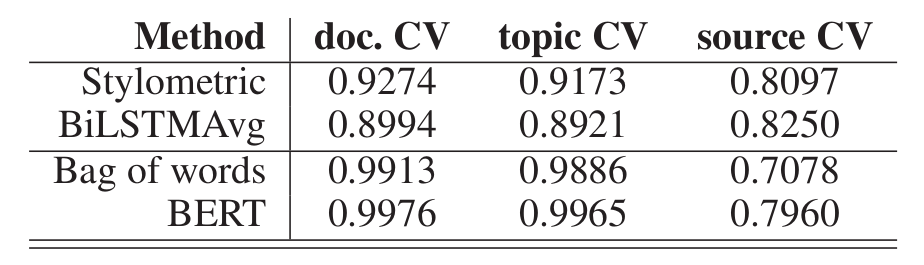
\includegraphics[scale=0.3]{img/styled_model_result.png}
	\caption{Classification accuracy of our stylometric and neural classifiers compared to baselines in three evaluation scenarios, simulating, respectively, a new document from known sources and topics, a document from unknown topic and a document from unseen source. \cite{przybyla2020capturing}}
\end{figure}

The obtained results shows that stylometric based classifier loses 10\% of the accuracy on unseen sources even if it has more consistent performance over evaluation scenarios. Piotr Przybyła explains this drop in accuracy by assuming that the model specialize in the style of individual sources rather than the general style of fake news. Nevertheless, he was able to prove that his model takes into account the affective words in order to classify fake news.
\section{Knowledge graph based fake news detection \cite{mayank2021deap} \cite{gad2019tracy}}
Studying the \textit{"DEAP-FAKED"} paper published in 2021 by \textit{Mohit Mayank}, \textit{Shakshi Sharma} and \textit{Rajesh Sharma}, it turned out that by exploiting techniques related to network analysis, Natural Language Processing (NLP) and the implementation of Graph Neural Networks (GNNs) we can detect fake news with an F1 score of 88\%.\\

The \textit{"DEAP-FAKED"} consists of three individual components:

\begin{itemize}
\item \textbf{News encoder:} this component performs the contextual encoding of news title. trying both unidirectional and bidirectional sequence encoders, they implemented a 2-layer stacked biLSTM as the main subcomponent the news encoder.
\item \textbf{Entity encoder:} this component identifies the named entities present in the news title and encodes the individual entities using knowledge graph (KG).
For example, a news title with text \textit{"US Officials See No Link Between Trump and Russia"}, contains two entities \textit{"Trump"} of person type and \textit{"Russia"} of geolocation type.
The framework includes relevant entities in the news then encodes them. They used Wikidata, an open-source KG, as the source to match the entities and ComplEx KG embedding technique to embed entities.
\item \textbf{Classification Layer:} this component consolidates the news encoder's and entity encoder's representations to perform the final downstream Fake News classification learning.
In this framework, the two representations are concatenated to create a super representation of the news content and entities. This representation is then passed to further non-linear activated layers with decreasing layer dimensionality. The final layer consolidated the information into a single dimension which is activated by a sigmoid layer, where the final output represents the probability of the news as either true or fake.
\end{itemize}

\begin{figure}[H]
	\centering
	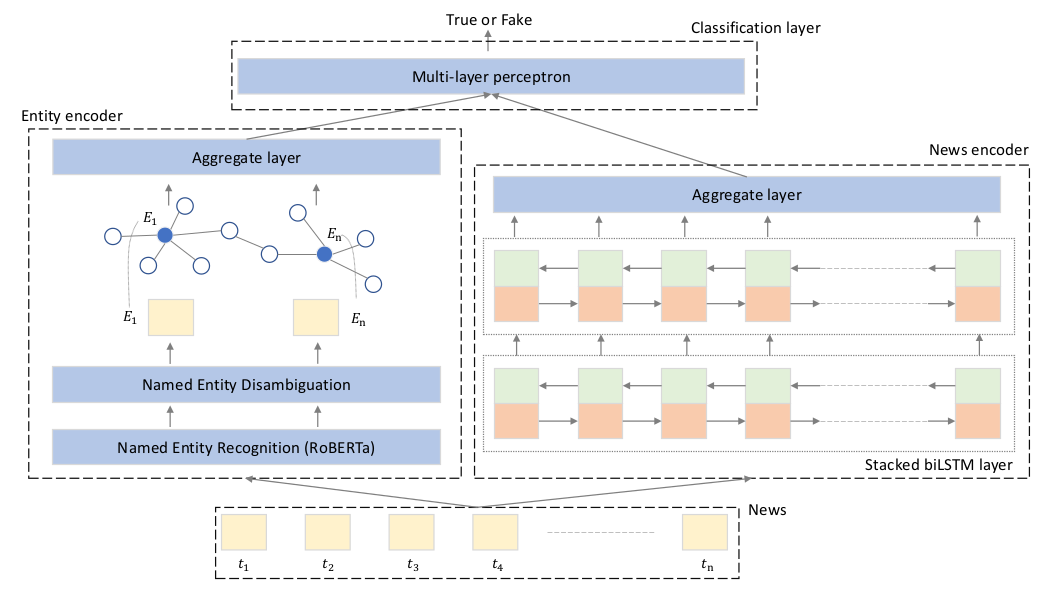
\includegraphics[scale=0.45]{img/deap_fake_framework.png}
	\caption{Illustration of the proposed DEAP-FAKED framework. The left sub-figure shows the entity encoder module. The right sub-figure shows the news encoder module. The top sub-figure is the Fake News classifier module. The bottom shows the tokenized news as the input to the entity encoder and news encoder. \cite{mayank2021deap}}
\end{figure}

The dataset used for \textit{DEAP-FAKED} framework can be described as following:

\begin{itemize}
\item \textbf{Fake News dataset:} The first dataset is the Kaggle Fake News dataset, which consists of 20,387 news items, having a near equal combination of true and Fake News. The news covers several domains such as Politics, Business, and Technology.
The complete pre-processing step brought down the news item count to  $\sim$14k with a distribution of 60\% - 40\% of true and Fake News classes, respectively.They called this dataset KFN-UB.\\
The second dataset is CoAID, which contains diverse COVID-19 healthcare misinformation, including Fake News from websites and social platforms. CoAID includes 4,251 news items. After pre-processing it only 632 news item and called CoAID-UB.
\item \textbf{Knowledge Graph:} the framework uses Wikidata5M as a knowledge graph, it is created by only considering the "valid" facts, where the validity is confirmed if all entities and relations in the fact have a Wikipedia article and long description.
\end{itemize}

As for the evaluation procedure, they chose five baseline models for comparison with \textit{DEAP-FAKED} framework: ExtraTreeClassifier, LSTM, SentRoBERTa, StackedBiLSTM, and StackedBiLSTM.

\begin{figure}[H]
	\centering
	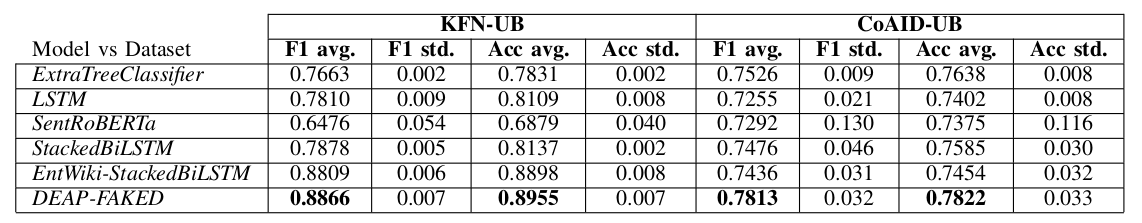
\includegraphics[scale=0.4]{img/deap_faked_evaluation.png}
	\caption{Performance score of the models detailed in the paper is presented here. For each of the dataset, we report F1 macro and Accuracy metric values. We present average and standard deviation of the performance observed after performing 3 trials with different starting seed. For both the datasets, DEAP-FAKED reports the best performance value. \cite{mayank2021deap}}
\end{figure}

As evident by the results, \textit{DEAP-FAKED} reports the highest score on both of the datasets.


\section{Hierarchical Propagation based fake news detection \cite{shu2020hierarchical} \cite{castillo2011information}}
In a paper wrote by \textit{Kai Shu}, \textit{Deepak Mahudeswaran}, \textit{Suhang Wang}, and \textit{Huan Liu} with the name of \textit{Hierarchical Propagation Networks for Fake News Detection: Investigation and Exploitation}, the detection of fake news can be done by looking at the correlation between news and the hierarchical characteristics of a social network.\\

The datasets used for this study were the public fake news repository \textit{FakeNewsNet} \cite{shu2018fakenewsnet} that contains data related to different fact-checking websites that offers news content, social context and dynamic information. In addition, they used the data from fact-checking websites \textit{GossipCop} and \textit{PolitiFact} that contains news articles with labels annotated by professional journalists. News content includes meta attributes of the news like body text, he social context includes the related user interactions with the news like posting, sharing, commenting on Twitter, and dynamic information contains the timestamps of user's interactions.\\

After collecting all of this data, building a hierarchical propagation network was the next step. First of all they defined two major levels of the hierarchy: 

\begin{itemize}
\item \textbf{Micro-level:} involves users conversations towards news pieces on social media over time. It contains rich information of user opinions towards news pieces.
\item \textbf{Macro-level:} encompasses information on tweets posting pattern and information sharing pattern. It represents the global propagation of information through a cascade of re-tweets.
\end{itemize}

\begin{figure}[H]%
	\centering
	\begin{subfigure}{.5\textwidth}
		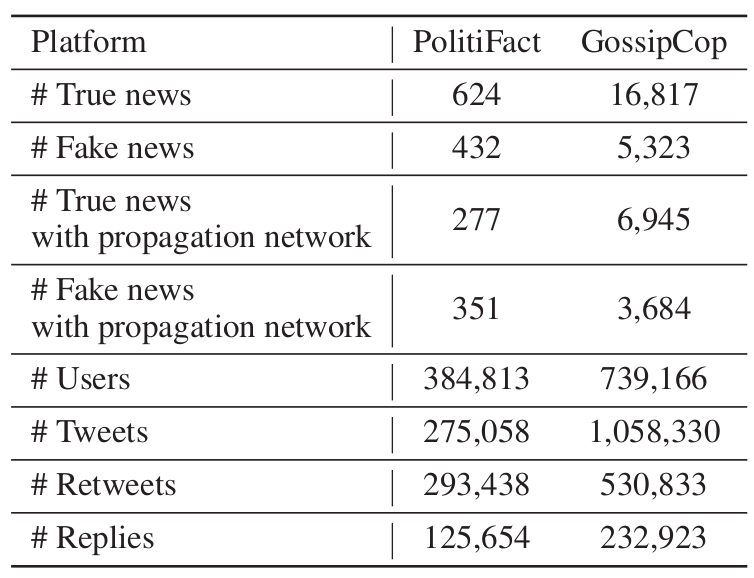
\includegraphics[width=.9\linewidth, height=7cm]{img/fake_news_net_content.png}
		\caption{The statistics of FakeNewsNet}
	\end{subfigure}%
	\begin{subfigure}{.5\textwidth}
		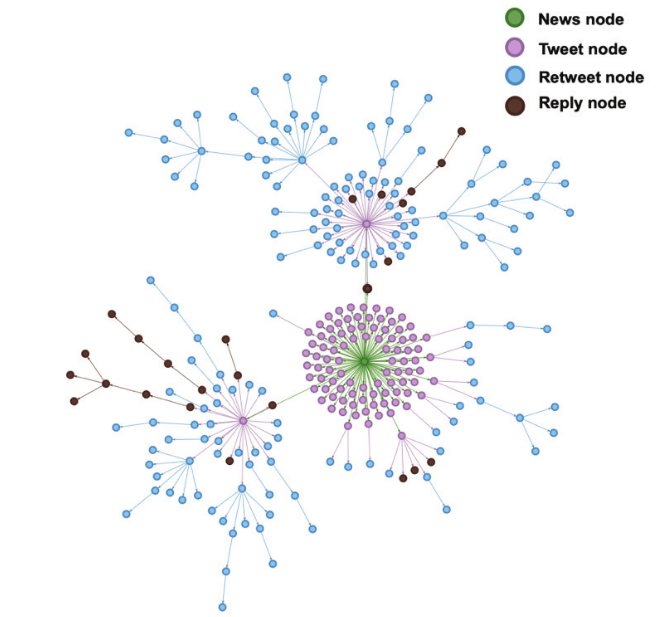
\includegraphics[width=.9\linewidth, height=7cm]{img/hierarchy_network.png}
		\caption{An example of the hierarchical propagation network of a fake news piece fact-checked by Politifact. It consists of two types: macro-level and micro-level. The macro-level propagation network includes the news nodes, tweet nodes, and retweet nodes. The micro-level propagation network indicates the conversation tree represented by cascade of reply nodes.}
	\end{subfigure}
	\caption{From the \textit{Hierarchical Propagation Networks for Fake News Detection: Investigation and Exploitation} paper}%
\end{figure}



In both these levels they used \textit{Structural Analysis} to identify patterns in conversations, \textit{Temporal Analysis} to understand the exchange of opinions in terms of time. For the Micro-level they added a \textit{Linguistic Analysis} to inference the sentiment of people around news pieces, thus obtaining linguistic features for statistical comparison.\\

To evaluate the performance of fake news detection of the model they choose randomly 80\% of news articles for training and the remaining 20\% for testing. The results shows high scores for both datasets:

\begin{figure}[H]
	\centering
	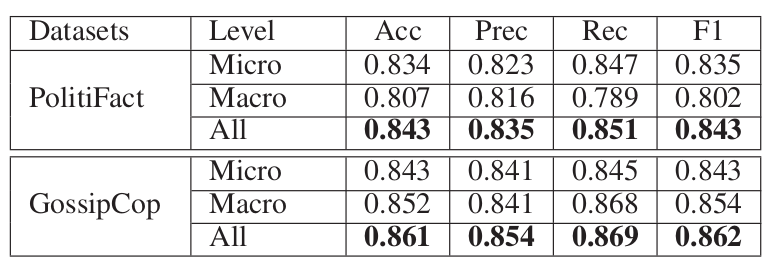
\includegraphics[scale=0.4]{img/hierarchical_evaluation_results.png}
	\caption{Evaluation of the model. \cite{shu2020hierarchical}}
\end{figure}


\section{Perplexity based fake news detection \cite{lee2021towards} \cite{lee2020misinformation}}
In March 2021, \textit{Nayeon Lee}, \textit{Yejin Bang}, \textit{Andrea Madotto}, \textit{Madian Khabsa}, and \textit{Pascale Fung} published a paper called \textit{Towards Few-Shot Fact-Checking via Perplexity} where they propose a new approach of the powerful transfer learning ability of a language model via a perplexity score. Using a method called \textit{few-shot learning}, they built a model that outperforms major class baseline models by more than 10\% on the F1-Macro metric score.\\

\begin{figure}[H]
	\centering
	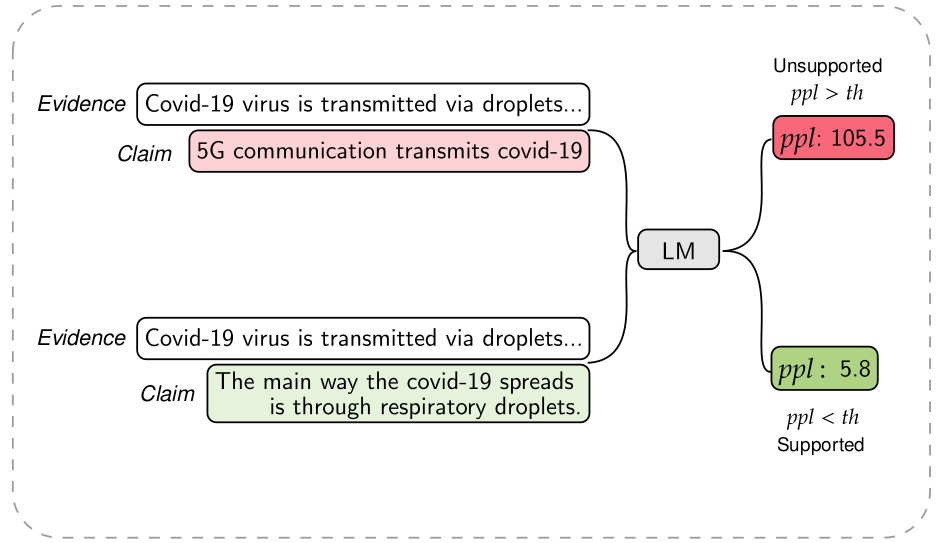
\includegraphics[scale=0.3]{img/perplexity_example.png}
	\caption{Illustration of our simple yet effective perplexity-based approach. Few-shot data samples are used to find the optimal perplexity threshold th that separates Unsupported claims from Supported claims. \cite{lee2021towards}}
\end{figure}

\textit{Few-Shot Learning} refers to the technique of feeding a machine learning model with a very small amount of training data to guide its predictions, like a few examples at inference time, as opposed to standard fine-tuning techniques which require a relatively large amount of training data for the pre-trained model to adapt to the desired task with accuracy.\\
In NLP, \textit{Few-Shot Learning} can be used with Large Language Models (LMs), which have learned to perform a wide number of tasks implicitly during their pre-training on large text datasets. This enables the model to generalize, that is to understand related but previously unseen tasks, with just a few examples.\\

Perplexity is a commonly used metric for measuring the performance of LMs. It is defined as the inverse of the probability of the test set normalized by the number of words:

\begin{figure}[H]
	\centering
	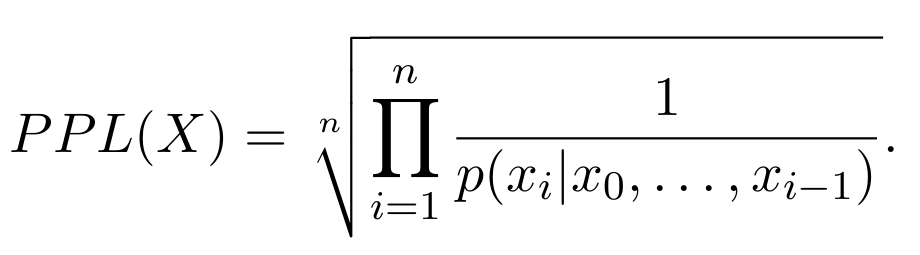
\includegraphics[scale=0.2]{img/perplexity_equation.png}
	\caption{Perplexity score. \cite{lee2021towards}}
\end{figure}

Another way of interpreting perplexity is as a measure of the likelihood of a given test sentence with reference to the training corpus.\\

In this paper the goal is to determine the veracity of a claim given some evidence, for this they define a {claim, evidence} pair. The label \emph{Supported} is assigned when relevant evidence exists that supports the claim, and \emph{Unsupported} label for the opposite case.\\
\emph{Unsupported} claims on average have higher perplexity than \emph{Supported} claims. For example, \emph{Supported} claim "Washing hands prevents the spread of diseases" has a perplexity value of 96.74, whereas the \emph{Unsupported} claim "All dogs speak English fluently" has a much higher perplexity value of 328.23. 

\begin{figure}[H]
	\centering
	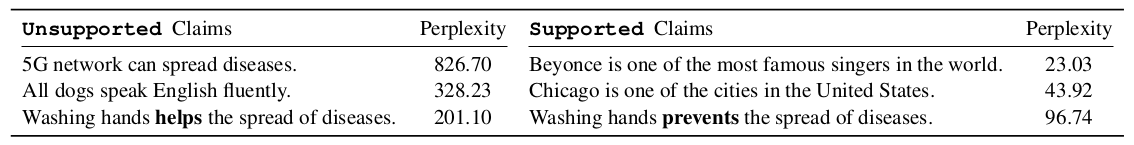
\includegraphics[scale=0.43]{img/supported_unsupported_perplexity.png}
	\caption{Relations between veracity of claim and perplexity. Unsupported claims have higher perplexity compared to Supported claims. Note that the perplexity score listed here is using GPT2-base on each of the claims. \cite{lee2021towards}}
\end{figure}

The datasets used in this experiment are:

\begin{itemize}
\item \textbf{Covid19-Scientific:} a new test set constructed by collecting COVID-19-related myths and scientific truths labeled by reliable sources like MedicalNewsToday, the Centers for Disease Control and Prevention (CDC), and the World Health Organization (WHO). The set contains 172 claims with labels \emph{(Supported, Unsupported)} obtained from the aforementioned reliable sources.
\item \textbf{Covid19-Social:} a collection of 340 COVID-19-related claims fact-checked by journalists from Politifact.com. Unlike the Covid19-Scientific dataset, it contains non-scientific and socially-related claims, such as "For the coronavirus, the death rate in Texas, per capita of 29 million people, we're one of the lowest in the country".
\item \textbf{FEVER:} Fact Extraction and Verification (FEVER) is a publicly released large-scale dataset generated by altering sentences extracted from Wikipedia to promote research on fact-checking systems.
\end{itemize}

For the models created for this perplexity based experiment they used one unidirectional LM and one masked LM:

\begin{itemize}
\item $PPL_{GPT2-B}$ : a single-parameter classifier based on perplexity from GPT2-base \cite{radford2019language} (unidirectional LM)
\item $PPL_{BERT-B}$ : a single-parameter classifier based on perplexity from BERT-base \cite{devlin2018bert} (Masked LM)
\end{itemize}

As for baseline models they finetuned pre-trained Transformer-based \cite{vaswani2017attention} in order to build a classifier, which is a common approach used to achieve many state-of-the-art results in the literature.\\

Moving to the experimental setup, they used the \textit{Few-Shot} technique in order to validate or train the models. Given $N_D$ as the size of the dataset $D$, we do an $n$-shot experiment with $n$ samples from $D$ as a "validation set" for our perplexity-based approach or as a "training set" for the fine-tuning approach, and the remainder ($N_D - n$) as a test set. For example in the 2-shot experiment using the Covid19-Social dataset (340 samples), we have two training samples and 338 test samples.\\
They took into consideration the accuracy and the F1-Macro metrics for the evaluation. Because the datasets are unbalanced, they mainly consider the F1-Macro score over accuracy as an overall evaluation.\\


\begin{figure}[H]
	\centering
	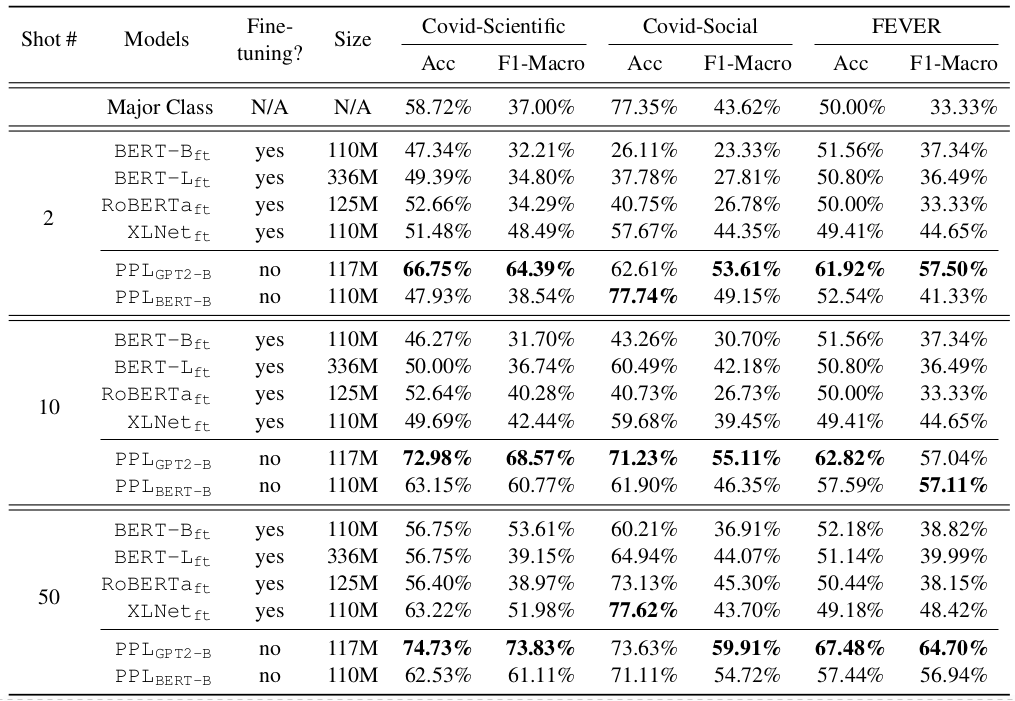
\includegraphics[scale=0.43]{img/few_shots_perplexity_evaluation.png}
	\caption{Results comparison among perplexity-based classifiers and fine-tuned classifiers in 2-shot, 5-shot and 10-shot settings across three different tasks. Models whose names start with PPL are our proposed perplexity-based classifiers. Major Class is a reference to evaluate classifier performance. All test results reported are mean values of three trials with randomly selected n-shot training samples from the dataset, where $n={2, 10, 50}$. \cite{lee2021towards}}
\end{figure}

We can observe that the perplexity-based classifiers, especially $PPL_{GPT2-B}$, outperform all Major Class baselines across all
tasks in all settings. For instance, $PPL_{GPT2-B}$ outperforms the Major Class by a great margin of
16\% and 36.8\% on accuracy and F1-Macro scores. Evidence conditioned perplexity scores are capable of providing signals regarding the veracity of the the given claim.

%\subsection{Other approaches}
%The interest of researches and social media companies in this area rises everyday, and other experiments and solutions were proposed such as:
%
%\begin{itemize}
%\item Fact verification using a large scale table \citep{chen2019tabfact}, where a large-scale dataset was constructed called \textit{TabFact} with 16k Wikipedia tables as the evidence for 118k human-annotated natural language statements, which are labeled as either ENTAILED or REFUTED. Then using the pre-trained language model BERT, called Table-BERT, to encode the linearized tables and statements into continuous vectors for verification achieving 68.1\% in accuracy metric.
%\item Web based fact verification, where 
%\end{itemize}

\chapter{Proposed method}
Most of the fact-checking algorithms today involving knowledge-based verification uses a traditional pipeline that puts in place a module for retrieving articles from an external source, another module for retrieving relevant sentences from each article and a last module for natural language inferencing (NLI) to classify a claim.

\begin{figure}[htp]
    \centering
    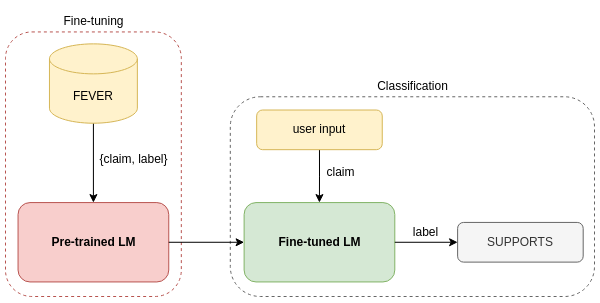
\includegraphics[scale=0.5]{img/processing_pipeline.png}
    \caption{Proposed method pipeline.}
    \label{fig:processing_pipeline}
\end{figure}


In this paper we present a method that is fully reliant on the powerfulness of today's best LMs. As illustrated in Figure \ref{fig:processing_pipeline}, we start by fine-tuning each model for the downstream task that is claim classification using the FEVER dataset, then each model is employed to assess the validity of new input claims. This approach takes into consideration only an internal knowledge source (FEVER) for fine-tuning, that is for the learning phase, which makes the prediction phase knowledge-free rather than utilizing external knowledge sources for retrieving articles and sentences.

It is also important to mention we only use LMs for classifying claims and not for generating evidence. We leave generating evidences with language models for future work.

\section{FEVER Dataset}
We will use the FEVER dataset as described before in section \ref{sec:fever}.\\
Since our mission is to classify claims to \textit{SUPPORTS}, \textit{REFUTES} or \textit{NEI} and not generating evidence, we omit the evidences information in the dataset. At that point we map each label to an integer: \{\textit{SUPPORTS} : 1, \textit{REFUTES} : 0, \textit{NEI} : 2\} and that is all we do as far as data pre-preprocessing goes.

\begin{table}[htp]
\centering
\resizebox{0.48\textwidth}{!}{%
\begin{tabular}{|c||c|c|}
\hline
\textbf{ID} & \textbf{Claim} & \textbf{Label} \\ \hline \hline
79044      & The Apple Store first opened in 2001.  & 1 \\ \hline
117129         & Adventure Time won an Oscar.    & 0  \\ \hline
55061           & Yamaha Corporation produces hardware.    & 2 \\ \hline
\end{tabular}
}
\vspace{0.4cm}
\caption{Examples of FEVER claims and labels.}
\label{tab:fever_example}
\end{table}

Finally, we split the dataset to training, validation and testing sets that we can use for LM fine-tuning and testing:

\begin{table}[htp]
\centering
\resizebox{0.48\textwidth}{!}{%
\begin{tabular}{|c||c|c|c|c|}
\hline
\textbf{Split} & SUPPORTS & REFUTES & NEI    & \textbf{Total} \\ \hline \hline
Train          & 80,035   & 29,775  & 35,639 & 145,449        \\ \hline
Val            & 3,333    & 3,333   & 3,333  & 9,999          \\ \hline
Test           & 3,333    & 3,333   & 3,333  & 9,999          \\ \hline
\end{tabular}%
}
\vspace{0.4cm}
\caption{Dataset split sizes for SUPPORTS, REFUTES and NOTENOUGHINFO (NEI) classes.}
\label{tab:fever_splits}
\end{table}

\section{Language Models}
The year 2018 has been an inflection point for NLP as Google introduced a LM called BERT (Bidirectional Encoder Representations from Transformers)\cite{devlin2018bert}. This model was described as state-of-the-art model that solves the most difficult tasks in NLP, it is also used today in Google's search engine for text completion and translation. BERT model can be fine-tuned with just one additional output layer to create state-of-the-art models for a wide range of tasks, such as question answering and language inference, without substantial task specific architecture modifications. From there many LMs were introduced that uses the same architecture as BERT but with small changes such as number of parameters and data on which the model was pre-trained.

\begin{figure}[htp]
    \centering
    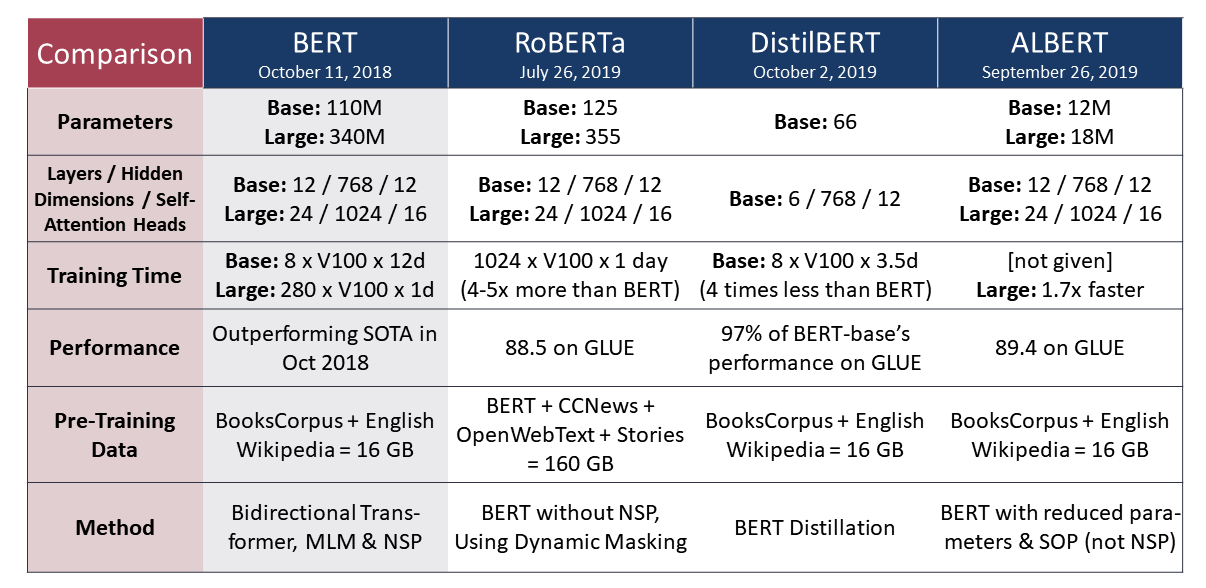
\includegraphics[scale=0.4]{img/lm_compar.png}
    \caption[Comparison]{Comparison of BERT, RoBERTa, DistilBERT, and ALBERT. \footnotemark}
    \label{fig:lm_compar}
\end{figure}
\footnotetext{\url{https://humboldt-wi.github.io/blog/research/information_systems_1920/uncertainty_identification_transformers/}}

In this paper we will classify claims by fine-tuning the following LMs:

\begin{itemize}
\item BERT-base-uncased \cite{devlin2018bert}
\item RoBERTa-base \cite{liu2019roberta}
\item DistilBERT-base-uncased \cite{sanh2019distilbert}
\item XLNET-base-cased \cite{yang2019xlnet}
\item ALBERT-base-v2 \cite{lan2019albert}
\item BigBird-RoBERTa-base \cite{zaheer2020big}\\
\end{itemize}

All of these LMs were trained on Wikipedia dataset containing cleaned articles. The datasets are built from the Wikipedia dump \footnote{\url{https://dumps.wikimedia.org/}} with one split per language. Each example contains the content of one full Wikipedia article with cleaning to strip markdown and unwanted sections (references, etc.). So in one way, all these LMs were trained on facts from Wikipedia, for example if we give the following input \textit{"Paris is the capital of [MASK]."} to BERT-base model, the output will be \textit{"Paris is the capital of France."} with a probability of 0.951.\\
Therefore the conjecture behind our method is that: by fine-tuning LMs that were pre-trained on Wikipedia, and by exploiting the already stored knowledge within these LMs, we can create a self-knowledge-independent fact-checking classifier.

\section{Experiment Protocol and Results}
\subsection{Experiment Setup}
As mentioned before, we conduct our experiment on the FEVER dataset using the splits in Table \ref{tab:fever_splits}. As for LMs fine-tuning we used one GPU, the NVIDIA RTX6000P-8C with 24Go of GDDR6 memory and a peak single precision floating point performance of 14,9 Tflops.\\

For all models we chose the following hyperparameters:\\

\begin{itemize}
\item Tokenizer max sequence length: 128
\item Output layer size: 3 (classes: 0, 1 and 2)
\item Activation function: GeLU
\item Learning rate: 3e-5
\item Optimization: Adam with linear decay
\item Loss function: Cross-Entropy
\item Epochs: 3
\item Training batch size: 20
\item Validation batch size: 20\\
\end{itemize}

These hyperparameters may not be optimal, but they were chosen after many different repeated experiments. Optimizing the models is left for future work.
\subsection{Evaluation Metric}
Most of the fact-checking methods that use FEVER dataset employ FEVER scoring\cite{thorne2018fever}, a metric that considers classification accuracy and evidence recall, but since we don't tackle the evidence problem in our approach, we rely on accuracy, recall, precision and F1-score of the model classification as metrics for evaluation.\\
In addition, we track other aspects of each LM such as training time, model size, and memory usage during the fine-tuning step in order to make an overall evaluation.
\subsection{Results \& Discussion}
The results of the six models are reported in Table \ref{tab:accuracy_res}. We can observe that our approach yields better results than FacebookAI's model and most of the traditional methods that involves external information retrieval modules.\\

\begin{table}[htp]
	\centering
	\resizebox{0.9\textwidth}{!}{%
	\begin{tabular}{c!{\vrule width \heavyrulewidth}cccccccc} 
	\bottomrule
	\textbf{Fine-tuned model} & \textbf{Label} & \textbf{prec} & \textbf{recall} & \textbf{~f1} & \textbf{accuracy} & \textbf{macro prec} & \textbf{macro recall} & \textbf{macro f1} \\ 
	\toprule
	\multirow{3}{*}{\textit{BERT-base-uncased}} & SUPPORTS & 0.55 & 0.78 & 0.64 & \multirow{3}{*}{\textbf{0.62}} & \multirow{3}{*}{0.63} & \multirow{3}{*}{\textbf{0.62}} & \multirow{3}{*}{\textbf{0.61}} \\
	 & REFUTES & 0.75 & 0.59 & 0.66 &  &  &  &  \\
	 & NEI & 0.61 & 0.47 & 0.53 &  &  &  &  \\ 
	\midrule
	\multirow{3}{*}{\textit{ALBERT-base-v2}} & SUPPORTS & 0.46 & 0.81 & 0.59 & \multirow{3}{*}{0.53} & \multirow{3}{*}{0.58} & \multirow{3}{*}{0.53} & \multirow{3}{*}{0.52} \\
	 & REFUTES & 0.77 & 0.46 & 0.58 &  &  &  &  \\
	 & NEI & 0.50 & 0.33 & 0.40 &  &  &  &  \\ 
	\midrule
	\multirow{3}{*}{\textit{DistilBERT-base-uncased}} & SUPPORTS & 0.54 & 0.78 & 0.64 & \multirow{3}{*}{0.61} & \multirow{3}{*}{0.63} & \multirow{3}{*}{0.61} & \multirow{3}{*}{\textbf{0.61}} \\
	 & REFUTES & 0.75 & 0.58 & 0.65 &  &  &  &  \\
	 & NEI & 0.60 & 0.47 & 0.53 &  &  &  &  \\ 
	\midrule
	\multirow{3}{*}{\textit{RoBERTa-base}} & SUPPORTS & 0.54 & 0.81 & 0.65 & \multirow{3}{*}{\textbf{0.62}} & \multirow{3}{*}{\textbf{0.64}} & \multirow{3}{*}{\textbf{0.62}} & \multirow{3}{*}{\textbf{0.61}} \\
	 & REFUTES & 0.75 & 0.59 & 0.66 &  &  &  &  \\
	 & NEI & 0.63 & 0.45 & 0.53 &  &  &  &  \\ 
	\midrule
	\multirow{3}{*}{\textit{BigBird-RoBERTa-base}} & SUPPORTS & 0.53 & 0.81 & 0.64 & \multirow{3}{*}{0.61} & \multirow{3}{*}{\textbf{0.64}} & \multirow{3}{*}{0.61} & \multirow{3}{*}{0.60} \\
	 & REFUTES & 0.75 & 0.58 & 0.66 &  &  &  &  \\
	 & NEI & 0.63 & 0.44 & 0.52 &  &  &  &  \\ 
	\midrule
	\multirow{3}{*}{\textit{XLNET-base-cased}} & SUPPORTS & 0.53 & 0.81 & 0.64 & \multirow{3}{*}{0.61} & \multirow{3}{*}{0.63} & \multirow{3}{*}{0.61} & \multirow{3}{*}{0.60} \\
	 & REFUTES & 0.74 & 0.59 & 0.65 &  &  &  &  \\
	 & NEI & 0.63 & 0.43 & 0.51 &  &  &  &  \\
	\bottomrule
	\textbf{Related work} & \textbf{Label} & \textbf{prec} & \textbf{recall} & \textbf{~f1} & \textbf{accuracy} & \textbf{macro prec} & \textbf{macro recall} & \textbf{macro f1} \\ 
	\toprule
	\multirow{3}{*}{\textit{BERT-large} \cite{lee2020language}} & SUPPORTS & 0.54 & 0.67 & 0.59 & \multirow{3}{*}{0.57} & \multirow{3}{*}{0.57} & \multirow{3}{*}{0.57} & \multirow{3}{*}{0.57} \\
	 & REFUTES & 0.62 & 0.55 & 0.58 &  &  &  &  \\
	 & NEI & 0.57 & 0.49 & 0.53 &  &  &  &  \\ 
	\midrule
	\textit{FEVER Baseline} \cite{thorne2018fact} & - & - & - & - & 0.49 & - & - & -\\
	\textit{Ohio State University} \cite{thorne2018fact} & - & - & - & - & 0.50 & - & - & -\\
	\textit{Columbia NLP} \cite{thorne2018fact} & - & - & - & - & 0.58 & - & - & -\\
	\textit{Papelo} \cite{thorne2018fact} & - & - & - & - & 0.61 & - & - & -\\
	\textit{UNC-NLP} \cite{thorne2018fact} & - & - & - & - & 0.68 & - & - & -\\
	\textit{DREAM} \cite{zhong2019reasoning} & - & - & - & - & \textbf{0.77} & - & - & -\\
	
	\end{tabular}%
	}
	\vspace{0.4cm}
	\caption{Classification metrics for each fine-tuned LM using our approach vs. BERT-large fine-tuned by FacebookAI team vs. other models based on knowledge graphs and/or traditional pipelines that uses FEVER dataset (we take into consideration only the accuracy of label classification and not the FEVER scoring system).}
	\label{tab:accuracy_res}
\end{table}

Specifically the fine-tuned \textit{RoBERTa-base} model surpasses the fine-tuned \textit{BERT-large} model created by FacebookAI in every metric. For instance our model achieved an accuracy score of 62\% and a macro precision score of 64\% which is an improvement of 5\% and 7\% respectively. Not only that, it is also worth mentioning that \textit{RoBERTa-base} has only 125 million parameters and 12 encoding layers in comparison to \textit{BERT-large} that has 340 million parameters and 24 encoding layers, thus rendering our model more efficient to train, to store and to implement.\\

The improvements in classification are presumably due to the fact that \textit{RoBERTa} is pre-trained on more data than \textit{BERT} as shown in Figure \ref{fig:lm_compar}. On the other hand, our fine-tuned \textit{BERT-base} model also achieved better results than FacebookAI's model which may be explained by the difference of hyperparameters choice.\\

Similarly, the fine-tuned \textit{RoBERTa-base} model achieved more accuracy score for label classification than most of the traditional pipelines. Therefore it puts our approach on the top-10 best fact-checking models that were published by FEVER community\cite{thorne2018fact} (without taking into consideration the evidence generation metric). It is also safe to say that the \textit{DREAM} fact-checking model is certainly superior than all our LMs as it achieved an accuracy score of 77\% which is 15\% higher. This is a proof that there is still much room for subsequent research and improvements.\\

Same as FacebookAI results\cite{lee2020language}, and upon examining the results of our fine-tuned LMs closely, we also find that all our LMs struggle immensely with the NEI category (lowest F1 scores) indicating that our current approach might also need specific modules to better tackle that category.\\
This was also confirmed when we plotted the confusion matrix of our models (for example \textit{RoBERTa-base} in Figure \ref{fig:confusion_matrix_roberta}).

\begin{figure}[htp]
    \centering
    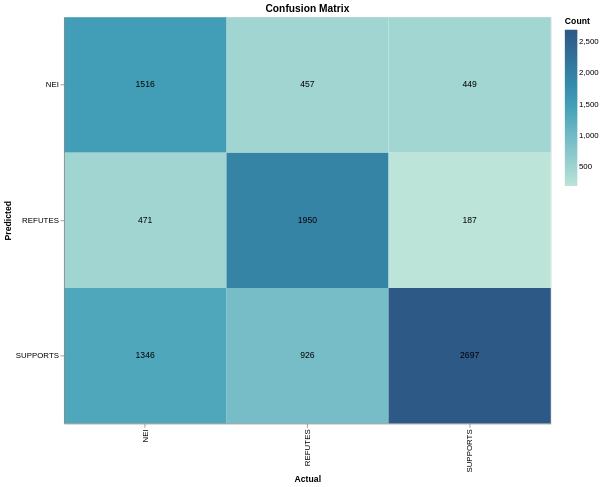
\includegraphics[scale=0.45]{img/confusion_matrix_roberta.png}
    \caption[Comparison]{Confusion Matrix of the fine-tuned \textit{RoBERTa-base} using test set.}
    \label{fig:confusion_matrix_roberta}
\end{figure}

Furthermore, the difference in classification performance between our LMs is not big considering the fact that each LM was pre-trained differently. The only model that performed poorly is \textit{ALBERT-base-v2}, it achieved only 53\% accuracy score and 52\% macro F1 score. This can be explained by the reduced number of the model's parameters (12 million vs. \textit{BERT}'s 110 million).\\

We can also see the differences between each LM during the training and the evaluation as illustrated in Figure \ref{fig:train_loss} and Figure \ref{fig:eval_loss}.

\begin{figure}[htp]
    \centering
    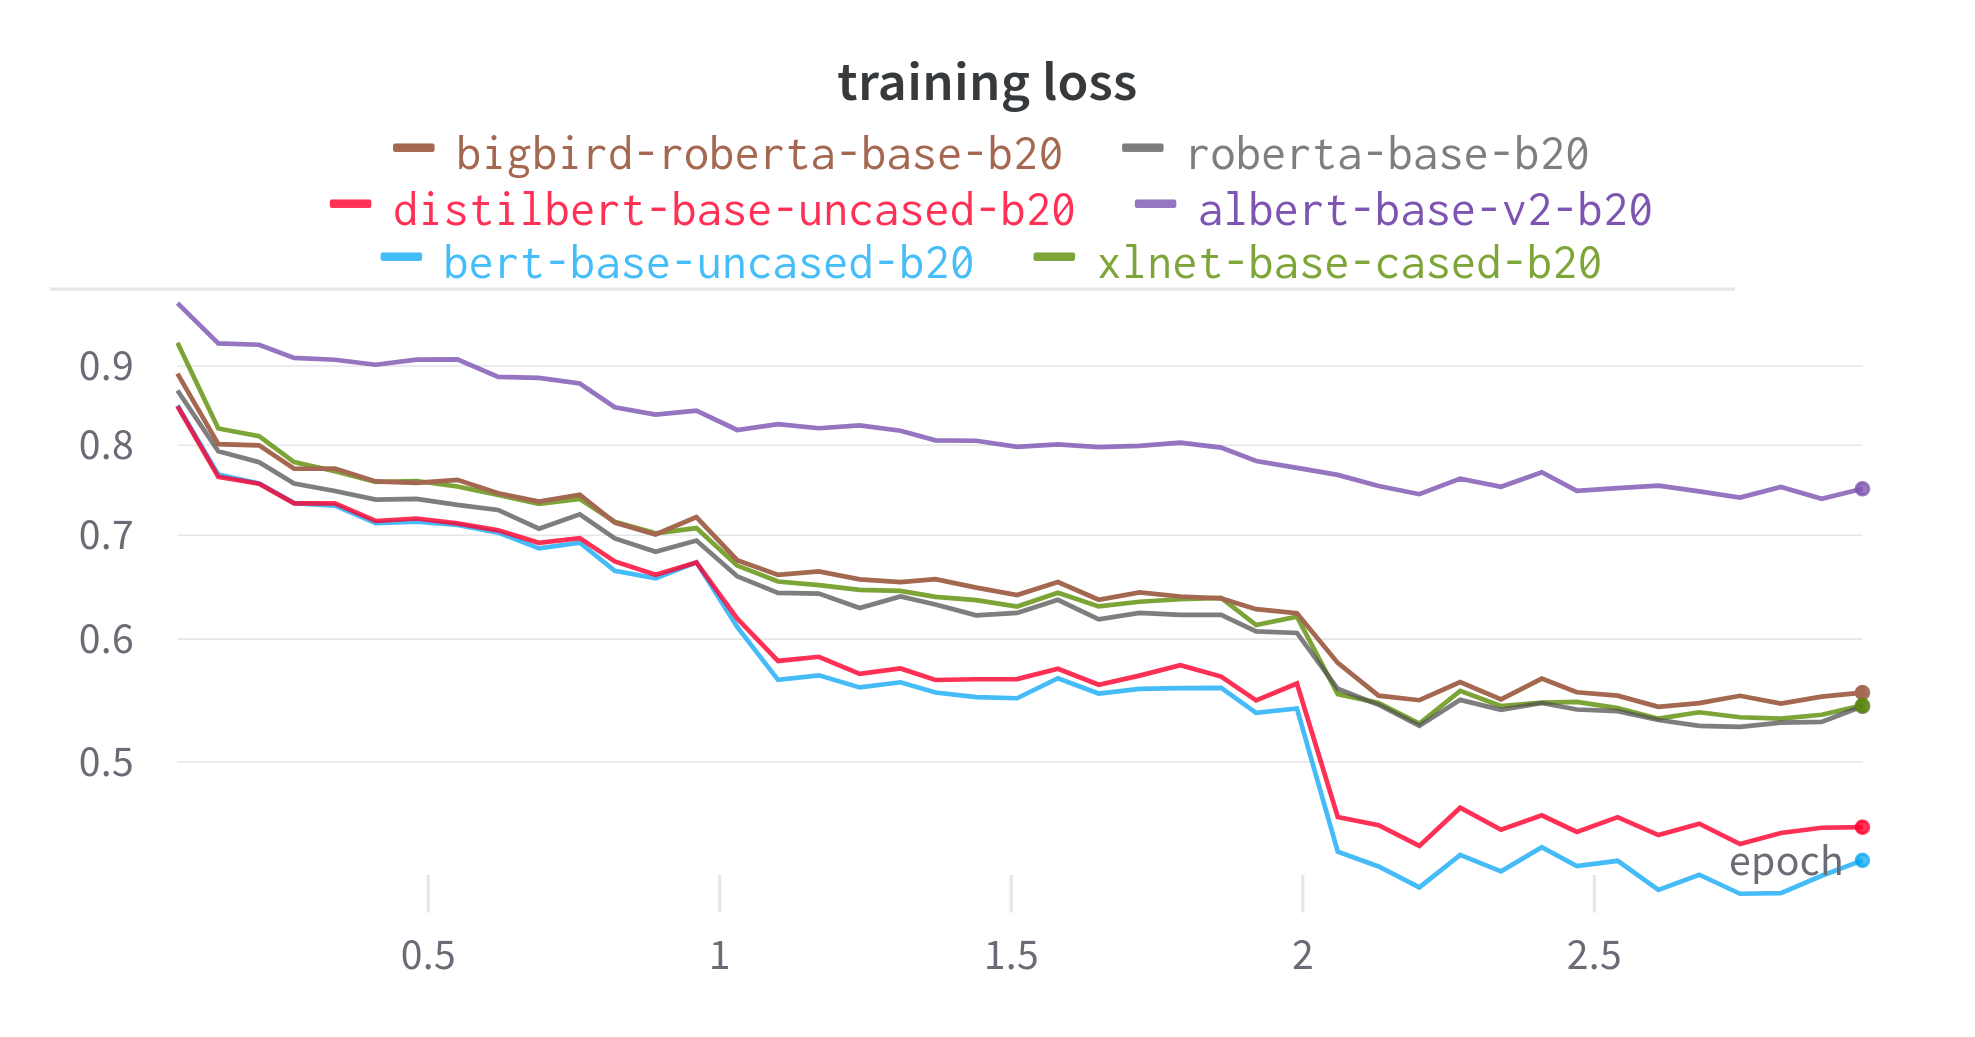
\includegraphics[scale=0.2]{img/train_loss.png}
    \caption[Comparison]{The Cross-Entropy Loss of each LM during training.}
    \label{fig:train_loss}
\end{figure}

\begin{figure}[htp]
    \centering
    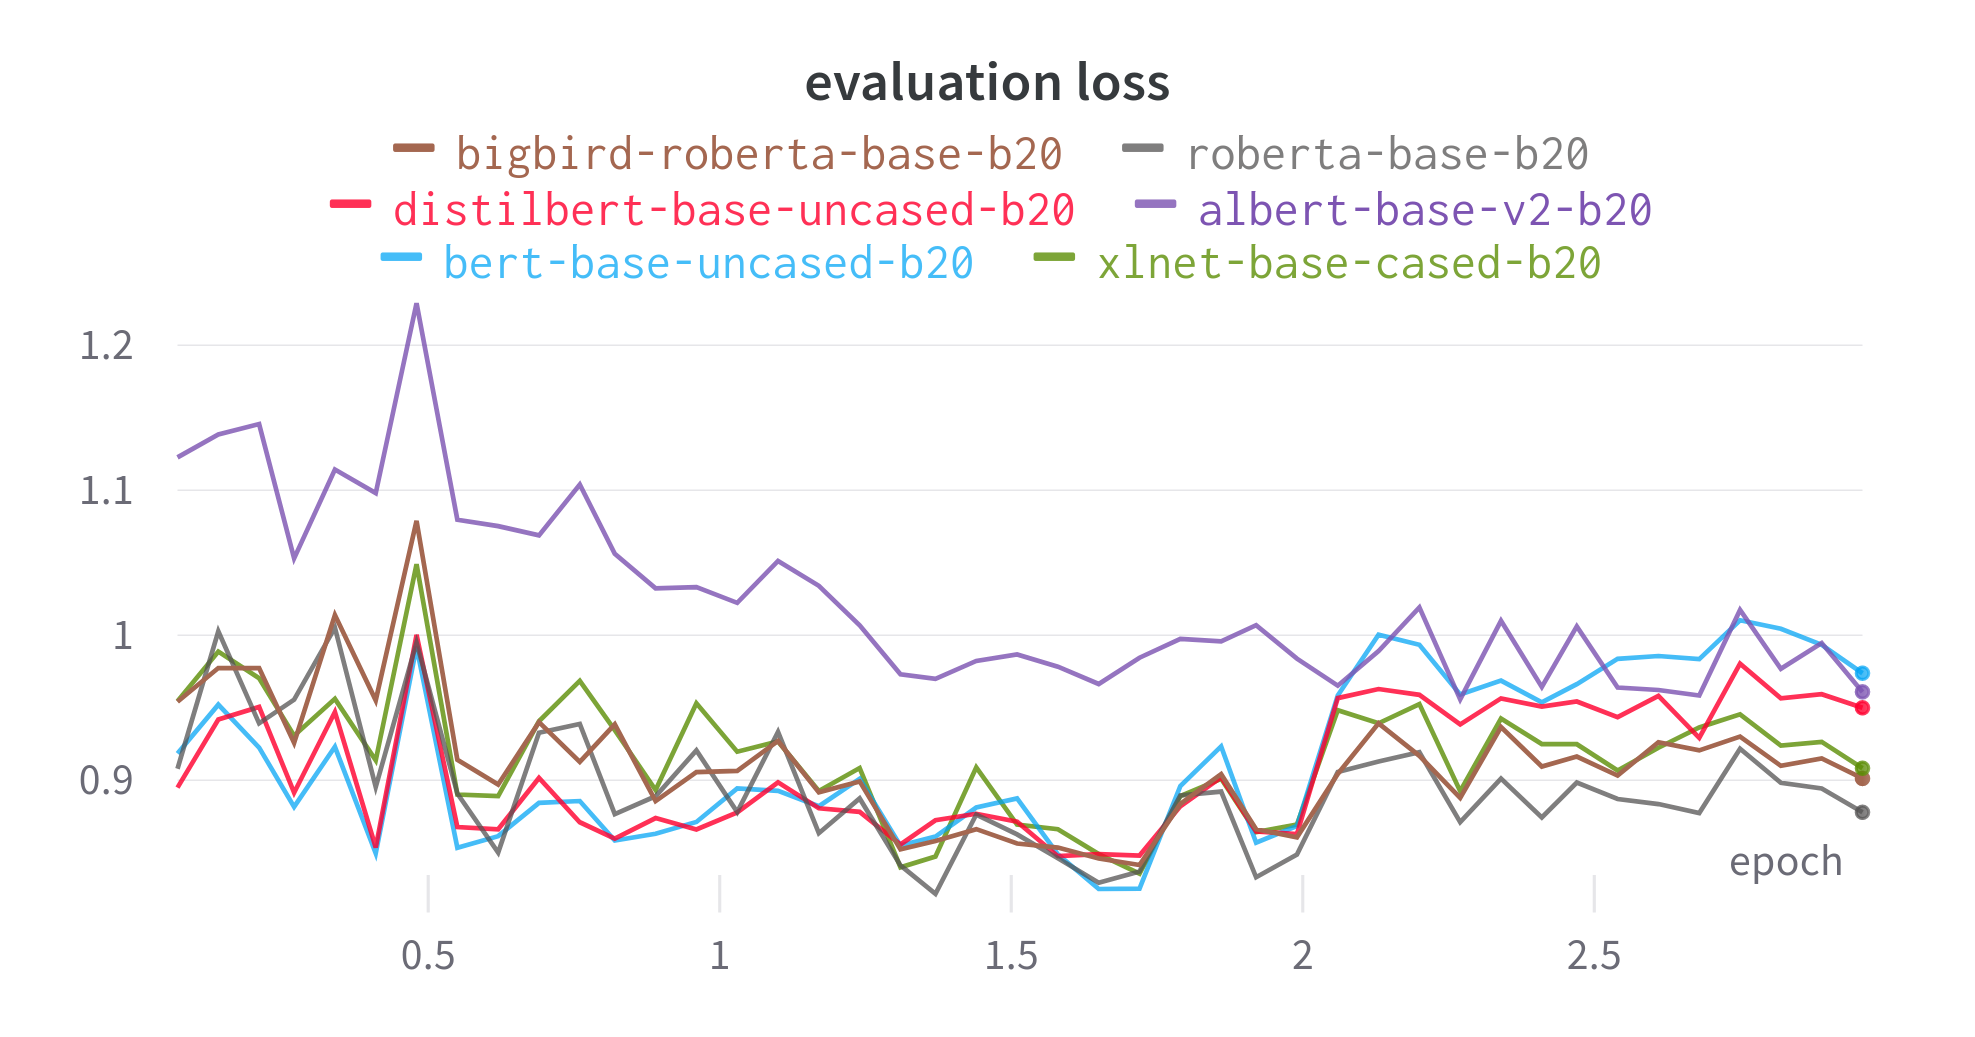
\includegraphics[scale=0.2]{img/eval_loss.png}
    \caption[Comparison]{The Cross-Entropy Loss of each LM during evaluation.}
    \label{fig:eval_loss}
\end{figure}

As expected, \textit{RoBERTa-base} model reached the lowest Cross-Entropy loss of 0.878 during evaluation while \textit{ALBERT-base-v2} sustained a higher loss of 0.961 during evaluation (also 0.75 during training). It is even more explicit in Figure \ref{fig:eval_mcc} and Figure \ref{fig:eval_acc} that \textit{ALBERT-base-v2} had the lowest Matthews correlation coefficient score (mcc) as well as accuracy score during evaluation.

\begin{figure}[htp]
    \centering
    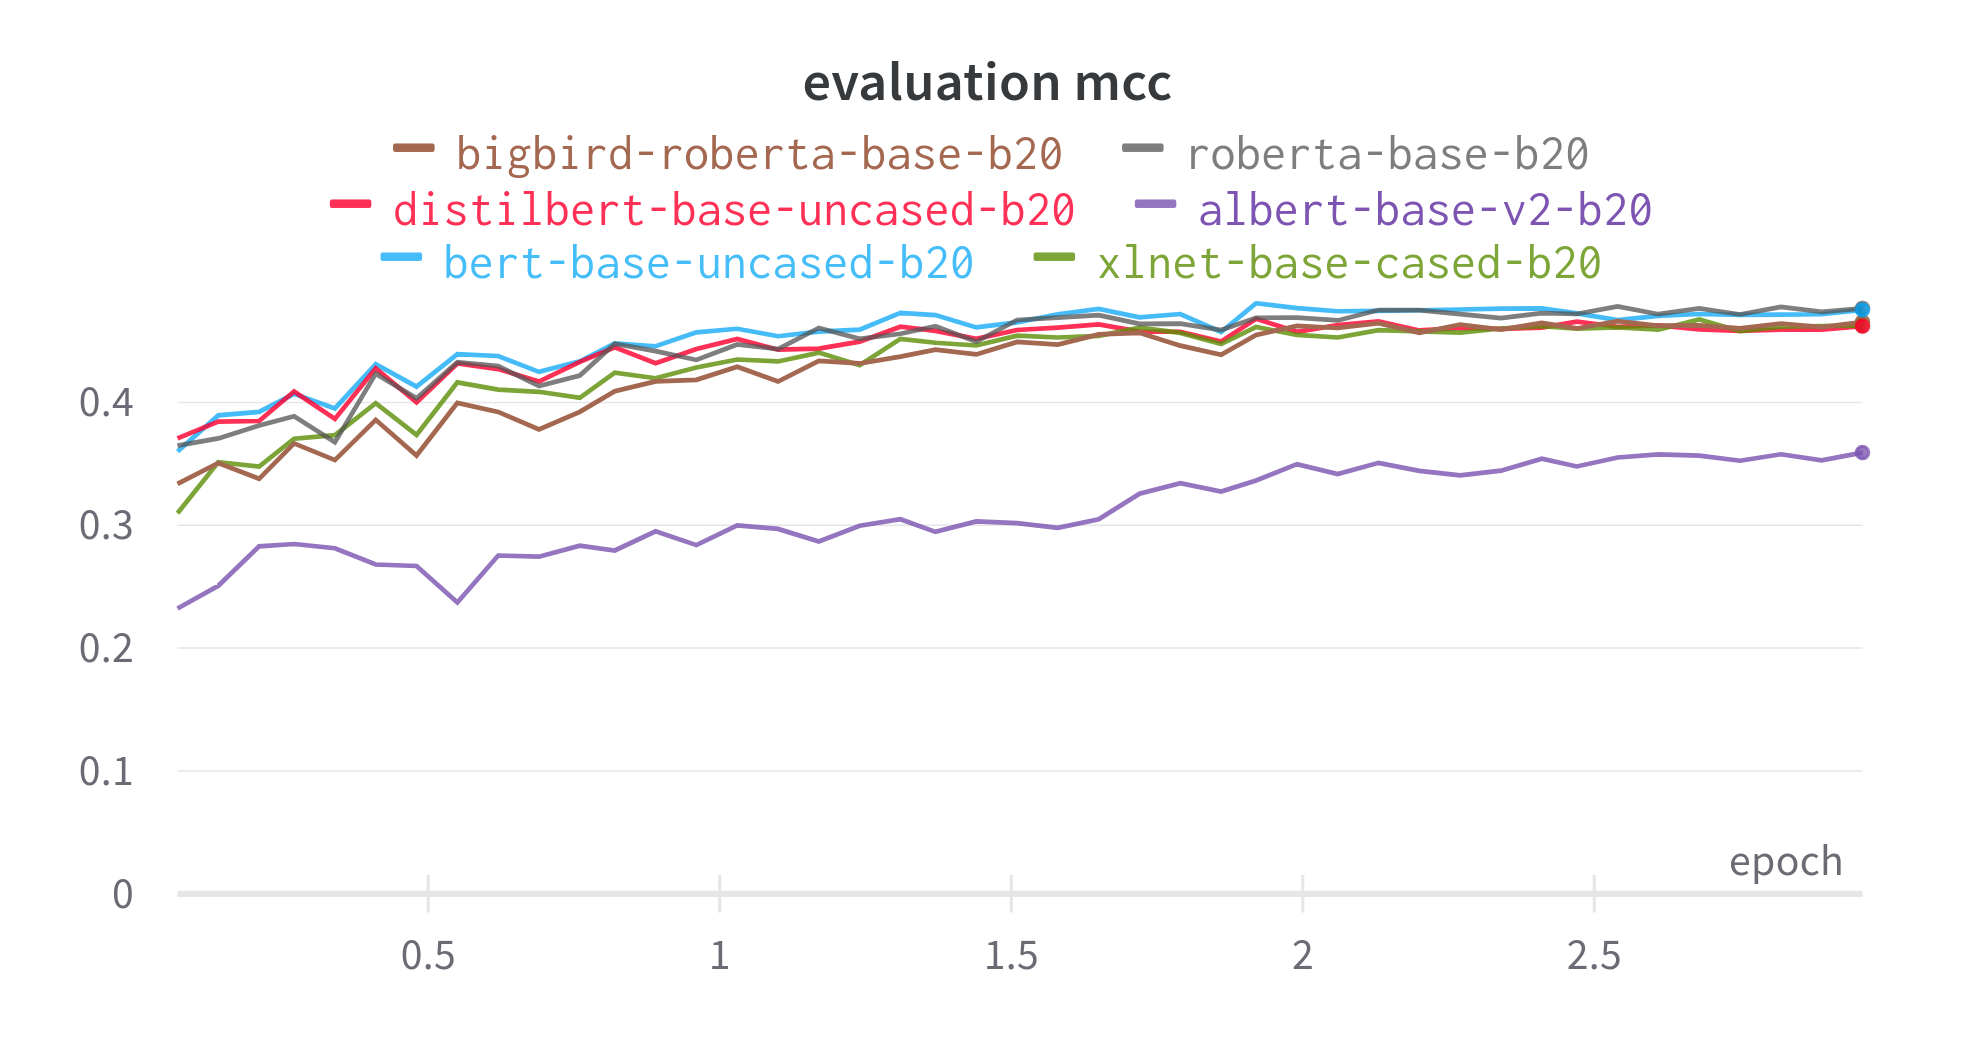
\includegraphics[scale=0.2]{img/eval_mcc.png}
    \caption[Comparison]{The Matthews correlation coefficient score of each LM during evaluation.}
    \label{fig:eval_mcc}
\end{figure}

\begin{figure}[htp]
    \centering
    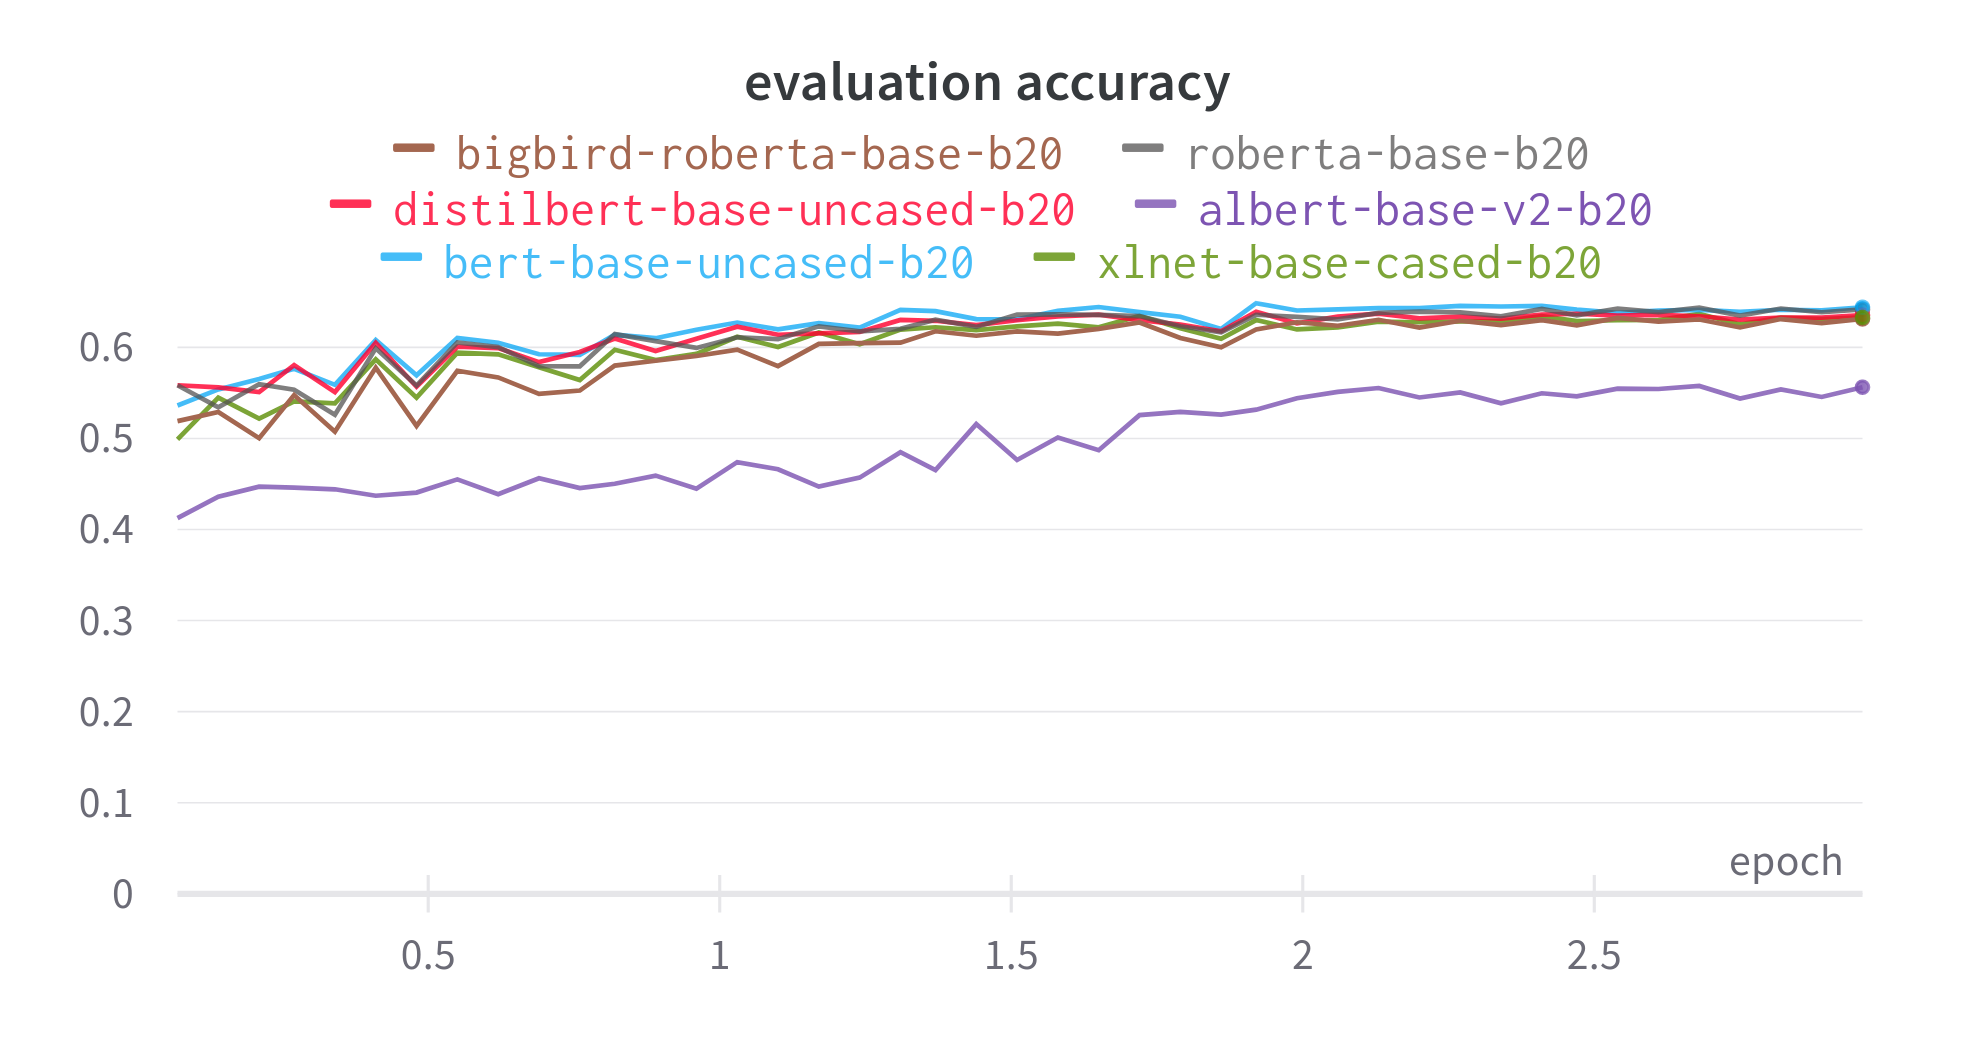
\includegraphics[scale=0.2]{img/eval_acc.png}
    \caption[Comparison]{The accuracy score of each LM during evaluation.}
    \label{fig:eval_acc}
\end{figure}

Even if the other LM reached the same accuracy and mcc as \textit{RoBERTa-base} during evaluation or a lower loss during training they did not perform as well in the test set which was demonstrated in Table \ref{tab:accuracy_res}.\\

Finally, it is also important to mention that training time differs from one LM to another (Figure \ref{fig:train_time}) as the number of parameters are not similar, for instance \textit{XLNET-base-cased} model spent 1h56m for training while \textit{RoBERTa-base} took 1h25m and achieved better results. The idea that we are trying to prove is we don't need a bigger model in order to achieve greater results for a downstream task like text classification.

\begin{figure}[htp]
    \centering
    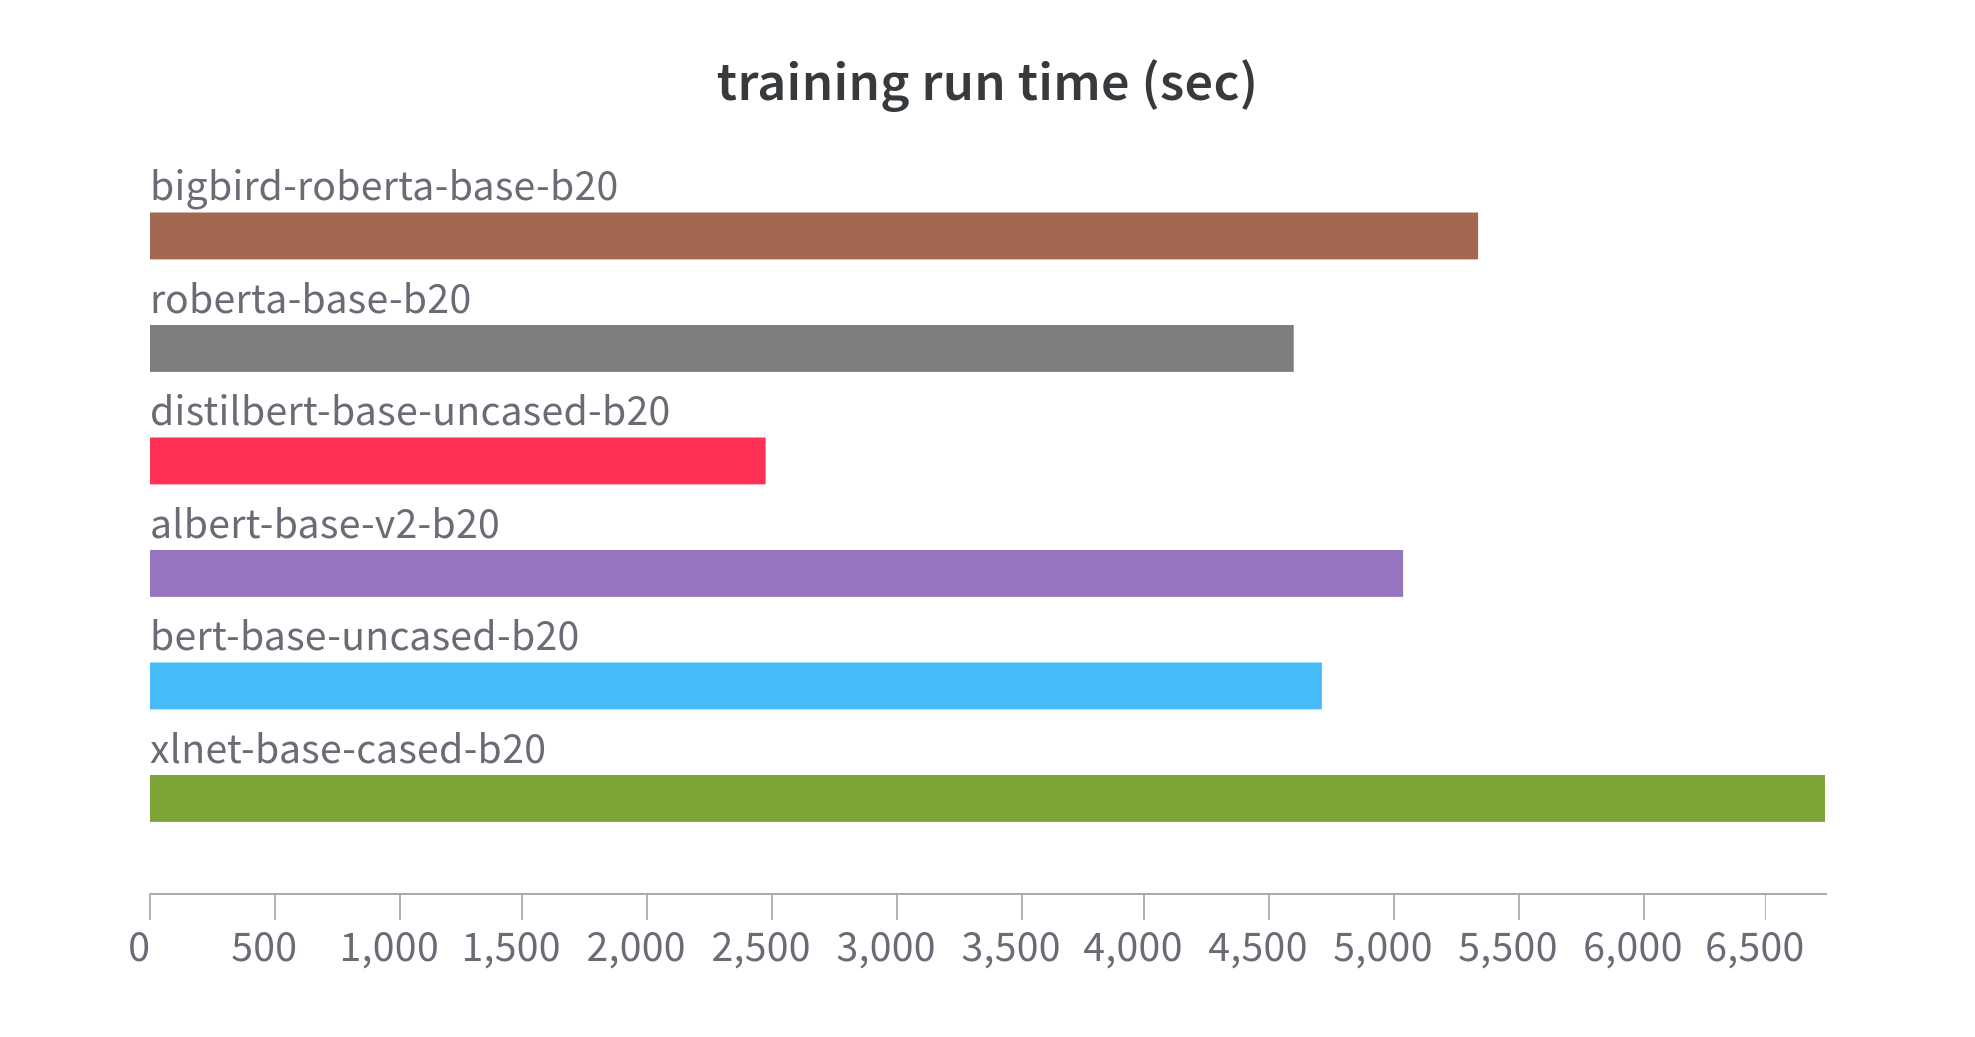
\includegraphics[scale=0.2]{img/train_time.png}
    \caption[Comparison]{Training time of each LM.}
    \label{fig:train_time}
\end{figure}

\section{Additional results}


\chapter{Conclusion \& Future Work}

In this paper, we explored the capabilities of language models to be fine-tuned and utilized for a downstream task that is fact-checking claims. We have successfully proven the effectiveness of pre-trained language models as an independent source of knowledge rather than implementing modules for external information retrieval adopted by traditional approaches. Our experiment conclusively yields results that surpasses most of the existing fact-checking methods both traditional and LM-based. Nevertheless, our approach does not beat state-of-art traditional models leaving us with more paths to explore in order to produce a reliable fact-checking engine.\\

In time to come, we plan to investigate solutions to deal with NEI category where our approach struggles. In addition, we will attempt to combine other models with our approach like credibility-based or style-based models, we will also implement evidence generation alongside claim classification in order to provide the user with reliable information.\\

All the articles and studies exploited in this literature research are fairly recent, which proves that fake news detection or fact-checking is one of the most urgent problems to deal with today in every society. As fake news about Covid-19 vaccines rocket through the roof in social media, the World Health Organization (WHO) said in a public tweet: We’re not just fighting a pandemic;
we’re fighting an infodemic.\\

Other companies like \textit{Facebook} are \textit{Twitter} are currently trying to make progress in fake news detection algorithms. We hope that during this project we can provide a new approach dealing with fake news propagation and contribute positively in this area.


\bibliographystyle{unsrt}
\bibliography{ref}


\end{document}
